%!TEX root = ../thesis.tex
%*******************************************************************************
%*********************************** First Chapter *****************************
%*******************************************************************************

\chapter{Introduction}  %Title of the First Chapter

% \ifpdf
%     \graphicspath{{Introduction/Figs/Raster/}{Introduction/Figs/PDF/}{Introduction/Figs/}}
% \else
%     \graphicspath{{Introduction/Figs/Vector/}{Introduction/Figs/}}
% \fi


% \nomenclature[z-cif]{$CIF$}{Cauchy's Integral Formula}                                % first letter Z is for Acronyms 
% \nomenclature[a-F]{$F$}{complex function}                                                   % first letter A is for Roman symbols
% \nomenclature[g-p]{$\pi$}{ $\simeq 3.14\ldots$}                                             % first letter G is for Greek Symbols
% \nomenclature[g-i]{$\iota$}{unit imaginary number $\sqrt{-1}$}                      % first letter G is for Greek Symbols
% \nomenclature[g-g]{$\gamma$}{a simply closed curve on a complex plane}  % first letter G is for Greek Symbols
% \nomenclature[x-i]{$\oint_\gamma$}{integration around a curve $\gamma$} % first letter X is for Other Symbols
% \nomenclature[r-j]{$j$}{superscript index}                                                       % first letter R is for superscripts
% \nomenclature[s-0]{$0$}{subscript index}                                                        % first letter S is for subscripts


%********************************** %First Section  **************************************
\section{The physics of QGP} %Section - 1.1 
\subsection{The strong interaction}
Since the discovery of atoms and their apparently smallest constituents (protons and neutrons) at least two topics have been deeply discussed by physicists for decades: are such particles fundamental (and if not how are they formed) and how do they interact?
The first big jump ahead towards the answer was performed in 1961 independently by Gell-Mann and Ne'eman with the the eight-fold theory, later developed further as the baryons octet and hyperions decuplet \ref{fig:gelmann}.
The organization of the particles was related to a symmetry group called $SU(3)$ which provides a triplet fundamental representation not observed in nature.
This hint, combined with the speculation that 8 or 10 particles were not likely all fundamental, lead to the introduction of more fundamental particles.

\begin{figure}[!ht]
\begin{center}
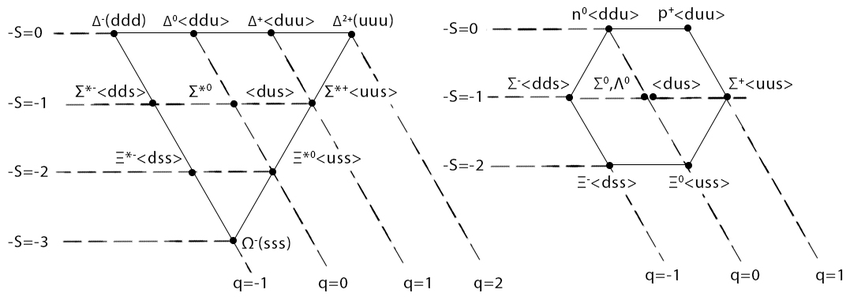
\includegraphics[width=0.8\linewidth]{Chapters/Introduction/Figs/eightfold_way.png}
\caption{Representation of the baryon decuplet (left) and octet (right) following the eightfold way approach for three kinds of quarks: up, down and strange. The horizontal levels represent the net strangeness number, while the diagonals (top left to bottom right) link baryons with the same electric charge.}
\label{fig:gelmann}
\end{center}
\end{figure}

They were later called quarks by Gell-Mann.
At a given point Gell-Mann and Zweig argued that, assuming the quarks' spin to be $1/2$, mesons could be explained as bound states of a quark and an antiquark, while baryons were a bound state of three quarks.
This choice lead to the peculiar electric charge of $\pm1/3$ and $\pm2/3$.
A last issue regarded the spin statistics theorem violation, solved by the introduction of an additional quantum number: the colour.
This was the birth of the quark model.
By assuming the hadronic matter is not fundamentally made of protons and neutrons they were able to organize in a elegant way the zoo of particles discovered during the $20^{th}$ century.

During the same years, Richard Feynman started thinking about a model useful for analyzing the hadrons produced in high energy physics experiments and capable of interpreting the radiation showers originating in ultra-relativistic collisions.
By introducing the partons and the parton distribution functions, Feynman was able to interpret the deep inelastic scattering on hadrons as the collision between the projectile and an inner constituent of the target, called parton \ref{fig:DIS}.

\begin{figure}[!ht]
\begin{center}
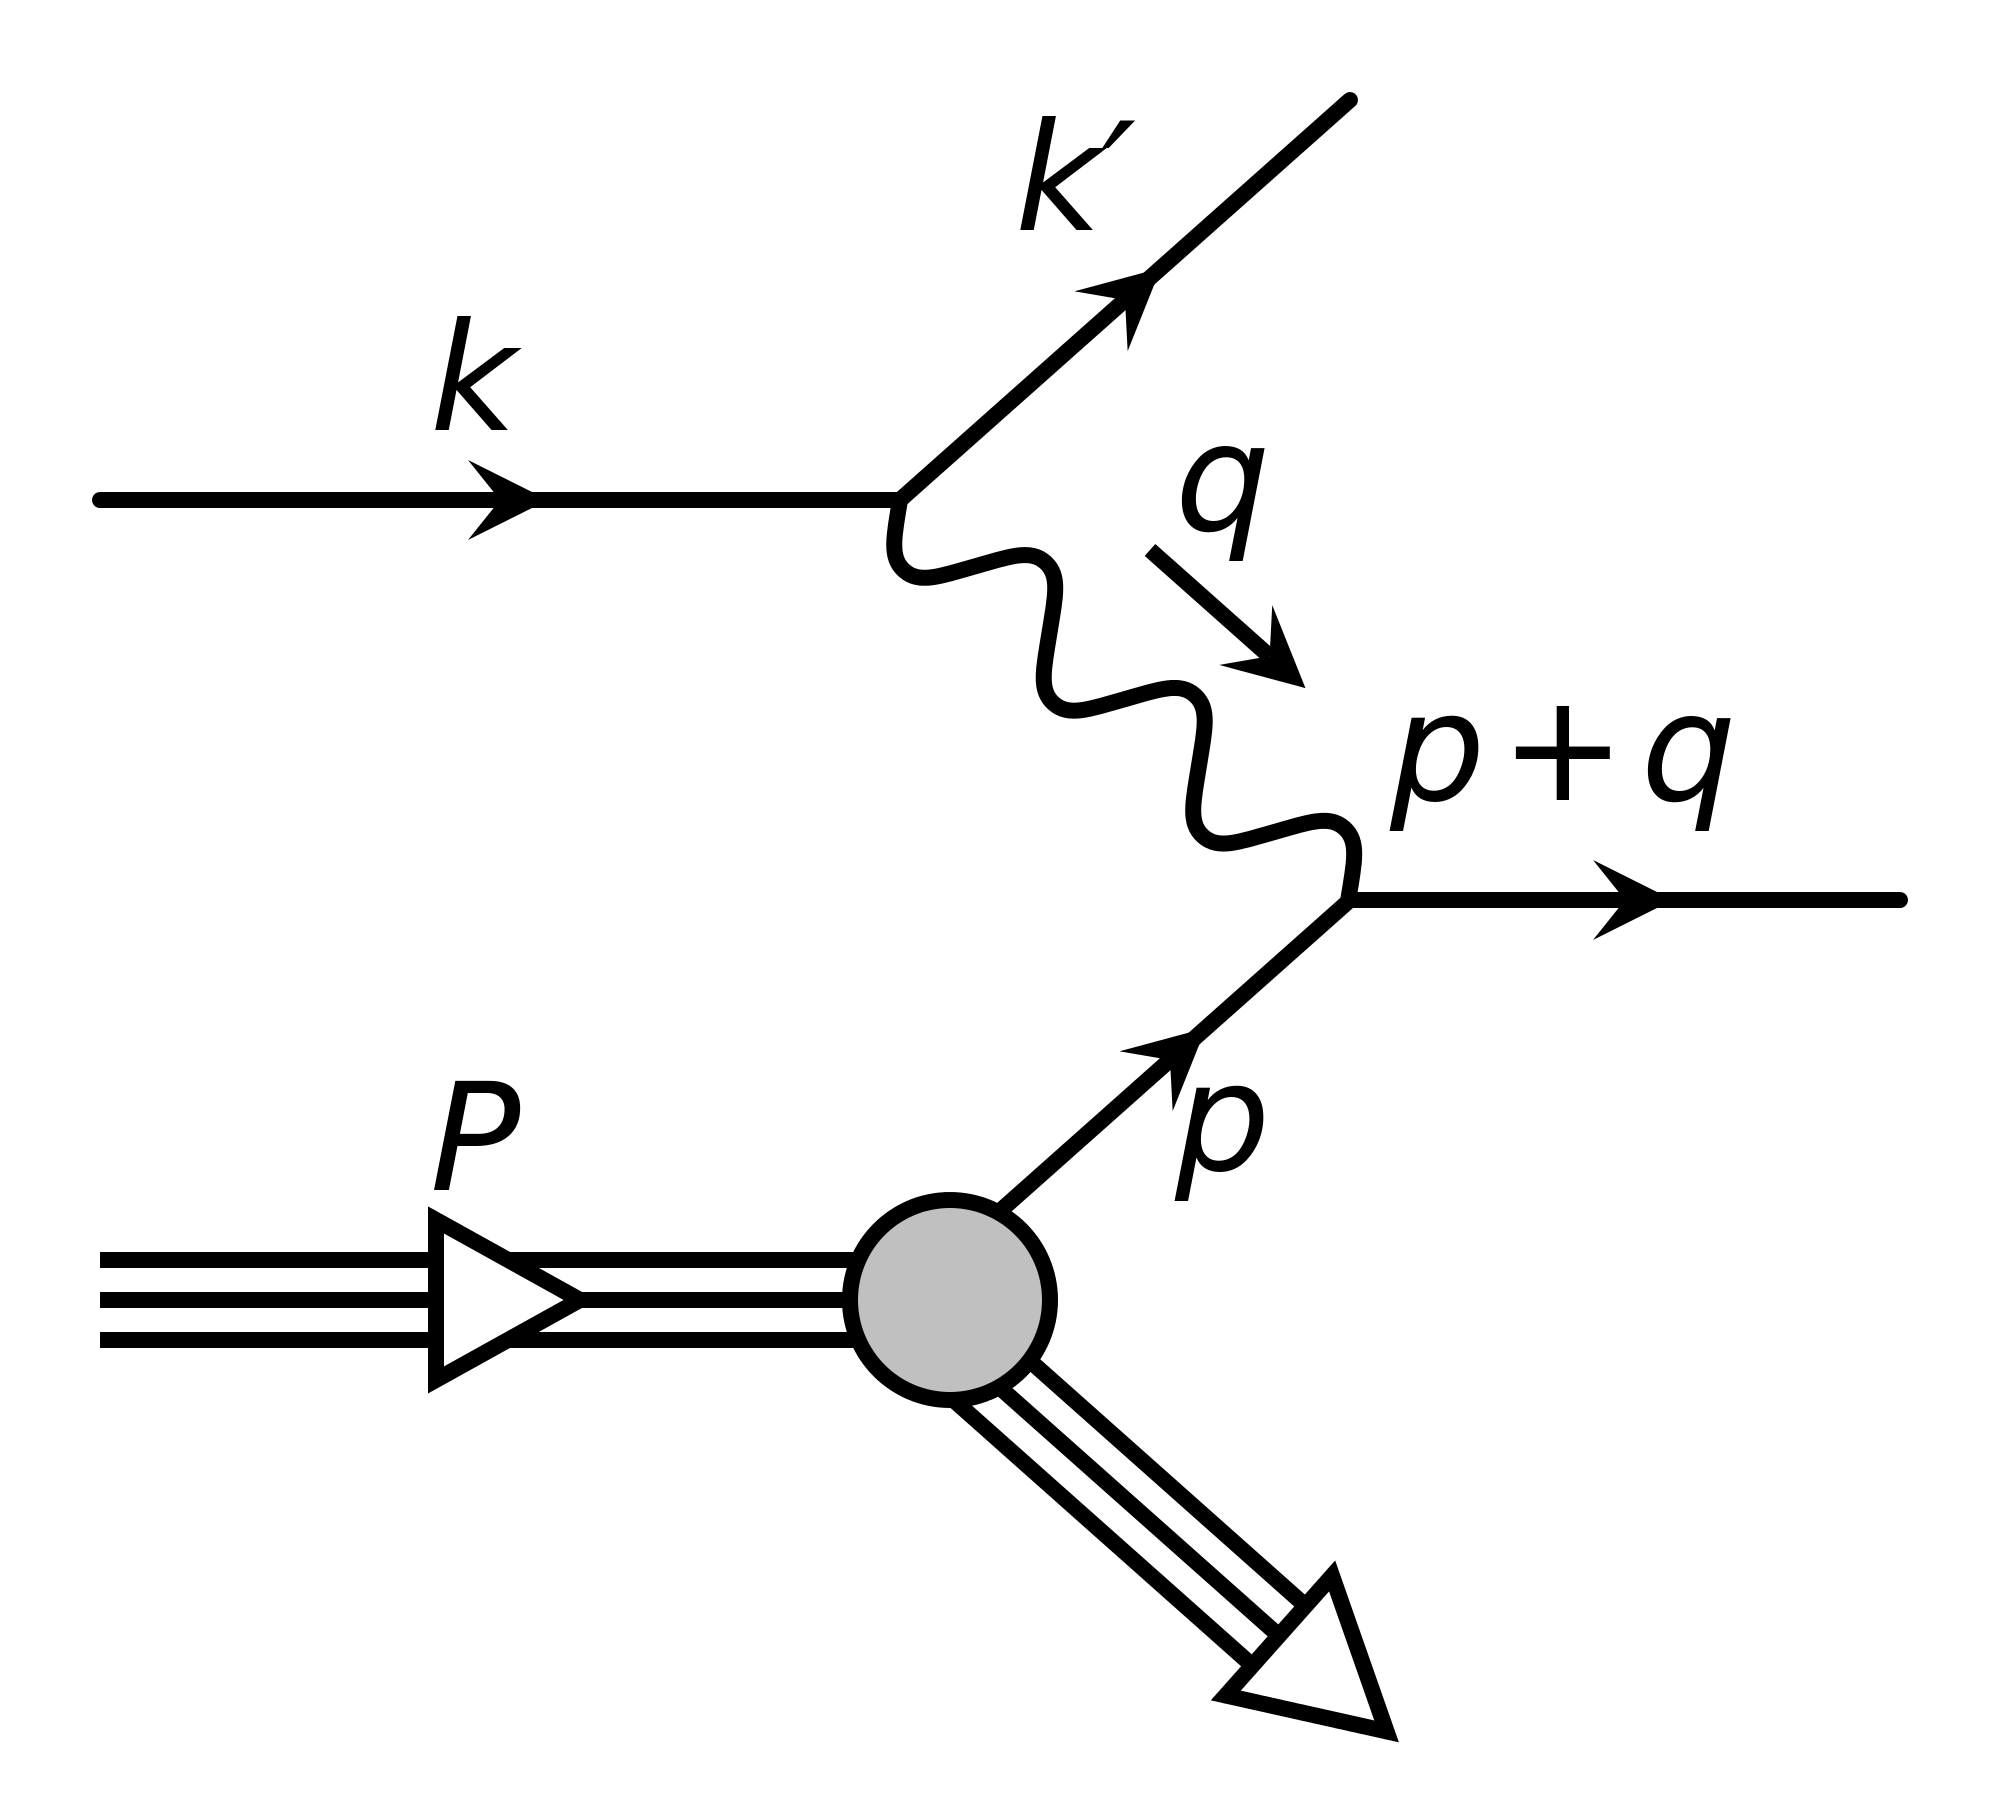
\includegraphics[width=0.5\linewidth]{Chapters/Introduction/Figs/DIS.png}
\caption{Cartoon of a deep inelastic scattering process between a projectile of momentum $k$ and $k'$and a parton of initial momentum $p$ belonging to a nucleon of initial momentum $P$. The interaction is mediated through the exchange of a boson of momentum $q$. The participant nucleons emerge from the interaction as an hadronic shower.}
\label{fig:DIS}
\end{center}
\end{figure}

Experiments of deep inelastic scattering performed at the Stanford Linear Accelerator Center (SLAC) between 1967 and 1973 pointed out a scaling behaviour, explained by Bjorken as a signature of the point like constituents of the proton.
Bjorken demonstrated that the functions which describe the structure of the nucleon neither depend on the transferred momentum ($Q^2$) nor on the energy transferred in the scattering ($\nu$), but on their ratio:

\begin{equation}
    x = \frac{Q^2}{2\cdot M \cdot \nu}
\end{equation}

The $x$ variable has no dimension and stands for the ration between the total momentum of the target and the fraction of that transported by the point-like constituent.


\begin{figure}[!t]
\begin{center}
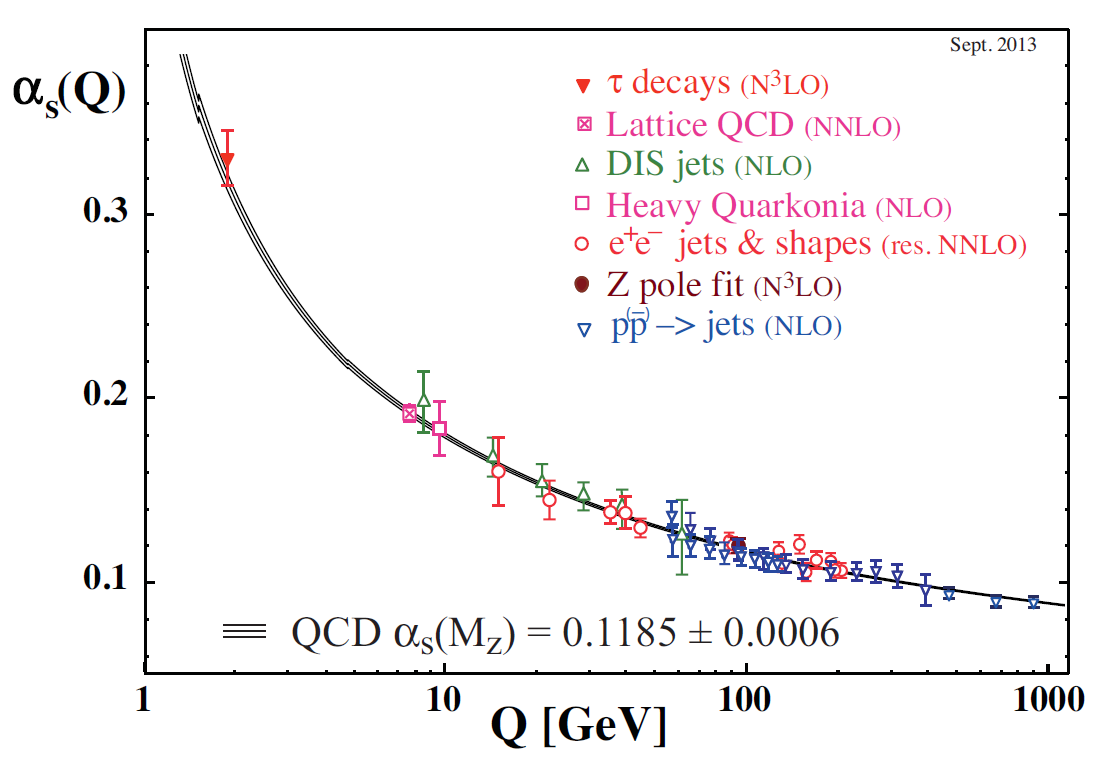
\includegraphics[width=0.85\linewidth]{Chapters/Introduction/Figs/QCD-running-coupling.png}
\caption{Plot of the running coupling constant of the strong interaction $\alpha_S$. The band has been computed using the standard model and several experimental points, obtained measuring the coupling from different processes, are shown.}
\label{fig:running}
\end{center}
\end{figure}

After few other proofs the Gell-Mann quarks and the Feynman partons turned out to be the same objects.
The answer to the first question was then well established (how are hadrons made?) when the physics community started tackling the second one regarding how do they interact.
The peculiarity of the new set of particles was the introduction of colour quantum number.
In 1973, in analogy with the Quantum Electro Dynamics (QED), the Quantum Chromo Dynamics (QCD) was proposed as the quantum field theory of the hadronic interaction.
The theory was supposed to be based on the existence of three colour charges and the non-Abelian simmetry group SU(3).
Eight massless generators represented the mediators of such interaction and were later called gluons.

The gluons are different with respect to the photons, since, as a effect of the non Abelian-ness of the theory, they carry a colour charge, making them auto interacting.
As a consequence the coupling constant of the strong interaction is defined as running, since it depends on the value of the transferred momentum $Q^2$\ref{fig:running}.
The running of the coupling constant leads to two peculiar proprieties, not found in any other fundamental interaction.
The strength of the interaction increases with distance.
This propriety leads to the confinement of quarks and gluons inside hadrons.

\begin{figure}[!t]
\begin{center}
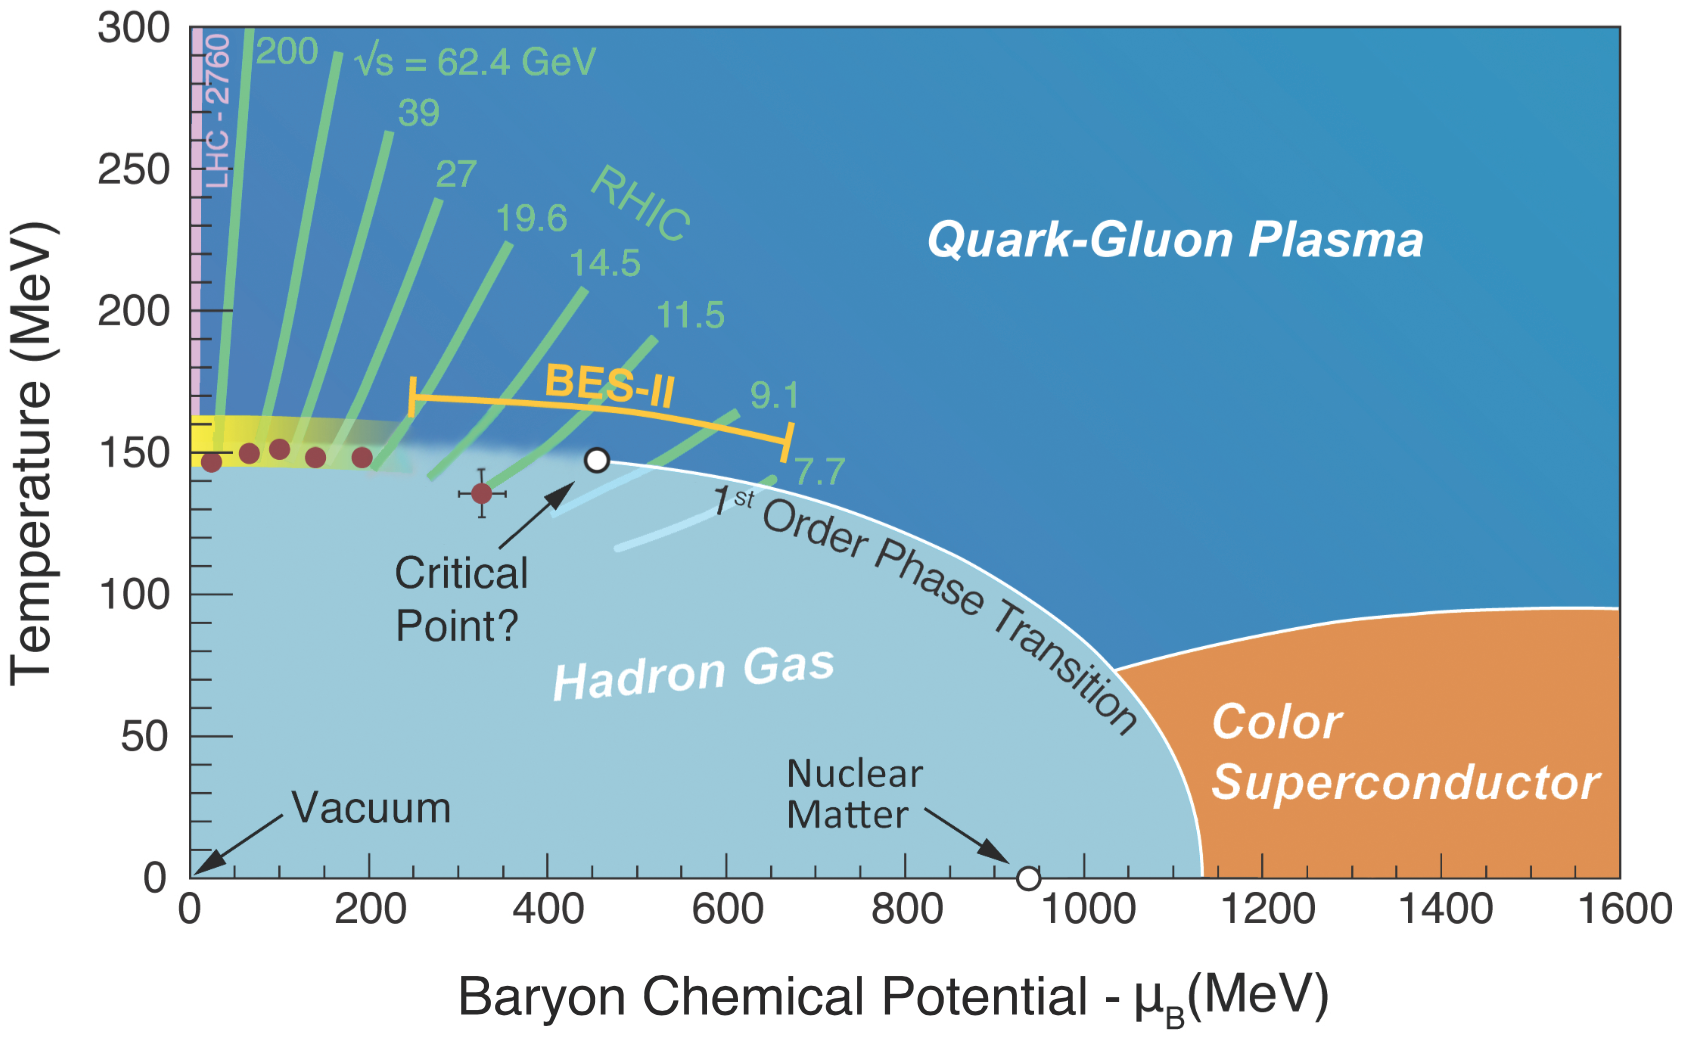
\includegraphics[width=0.85\linewidth]{Chapters/Introduction/Figs/QGPPhases.png}
\caption{Cartoon showing the main hadronic matter phases in a $(T,\mu_B)$ diagram.}
\label{fig:QGPPhases}
\end{center}
\end{figure}

\subsection{Quark Gluon Plasma}
In 1977 E. Shuryak coined the term Quark Gluon Plasma (QGP) to indicate a state of nuclear matter in which quarks and gluons are not confined anymore into hadrons.
From theoretical studies the main parameters determining the QGP evolution are the temperature (T) and the baryon-chemical potential ($\mu_B$), defined in a thermodynamical fashion as the differential of entropy with respect to the net baryon number.
Three main regions are spotted in the $(T,\mu_B)$ phase diagram \ref{fig:QGPPhases}:
\begin{itemize}
    \item At low T and low $\mu_B$ the nuclear matter is composed of hadrons behaving as a hadrons gas;
    \item At low T and high $\mu_B$ the nuclear matter degenerates to a gas of neutrons due to the collapse of hadronic structure. This state of nuclear matter is supposed to be present in the core of neutron stars;
    \item At high T and high $\mu_B$ the gas can be described as a gas of weakly interacting partons. Such behaviour is caused by the asymptotic freedom of QCD.
\end{itemize}
The extreme conditions needed for the QGP production are similar to the ones happened at the beginning of the universe evolution can be obtained in laboratory by means of ultra-relativistic heavy ion collisions.
According to the Big Bang model the conditions of high temperature and low baryon-chemical potential are supposed to be the ones of the early Universe.
At the beginning of the universe all the energy and matter were condensed in a tiny spatial region.
During the first microseconds of evolution, the universe started expanding from a condition of extreme energy density and temperature.
While expanding the energy density and the temperature started dropping.
Two transitions happened at $T\simeq160 MeV$ and $T\simeq100 KeV$: the hadron formation started at the first threshold, while small nuclei could survive after the second value.
The nuclear composition of early universe was fixed at that point: such phenomenon is called primordial nucleo-synthesis.
Only few minutes later, when the universe temperature dropped below $3000K$, the radiation decoupled from matter and the whole universe started becoming transparent.
The Cosmic Microwave Background (CMB) is the residual of the first radiation.

Studying the QGP evolution and its characteristics might lead to a better understanding not only of the strong nuclear interaction and the origin of hadrons masses, but also of the process of universe formation.

The best phenomenological model which can be cited to understand the artificial methodology to produce QGP is the bag model.
The two main hypotheses of this model are:
\begin{itemize}
    \item the quarks are massless particles put inside a bag of infinite dimension;
    \item the confinement originates from the balancing of the internal pressure exerted by quarks into the bag and an external pressure $B$;
\end{itemize}
The total energy of $N$ quarks confined in a spherical volume of radius $R$ is the sum of a kinetic term and a term related to the compensation by the external pressure $B$:
\begin{equation}
    E=\frac{2.04\cdot N}{R}\cdot \hslash c + \frac{4\pi}{3}\cdot R^3\cdot B
\end{equation}
The bag radius is determined by finding the minimum of energy of the system.
Such condition is obtained imposing the condition $dE/dR=0$.
\begin{equation}
\frac{dE}{dR}=-\frac{2.04\cdot N}{R^2}\cdot \hslash{h}c + 4\pi\cdot R^2\cdot B = 0
\end{equation}
The model allows one to compute confinement thresholds for various systems.
For example a baryon, composed by $N=3$ quarks and with $R=0.8 fm$ the external pressure becomes:
\begin{equation}
B^{1/4} = \frac{206 MeV}{\hslash c}
\end{equation}
Such value is the limit below which the confinement of the quarks inside the baryon happens.
If the internal pressure grows above such threshold the quarks start behaving as asymptotically free.
The internal pressure can increase in two ways:
\begin{itemize}
\item The increase of temperature causes an increase of kinetic energy of quarks inside the bag. In this situation the formed QGP is called "hot";
\item The increase of pressure is caused by the increase of baryon density achieved via compression. This scenario is possible in extremely dense objects such as neutron stars and is defined as "cold" QGP.
\end{itemize}

The heavy-ion collision experiments tackle the QGP production mainly trough the first approach, thank to the high energy available in the center of mass of the collision, while the use of heavy nuclei instead of light ones addresses the second method.
The bag model provides an estimation of the minimum temperature and energy density needed to produce the deconfined state.

The pressure required to produce a QGP out of a volume $V$ filled with massless quarks and gluons in which the net baryon number is null (equal number of quarks and anti-quarks) is computed as:
\begin{equation}
P = g_{tot}\cdot\frac{\pi^2}{90}\cdot T^4
\end{equation}
Where $g_{tot}$ is the total number of degrees of freedom for quarks, anti-quarks and gluons.
The pressure exceeds the external one at a temperature of around $145MeV$, a value similar to the lattice-QCD prediction of $160MeV$.
In addition, since the energy density is related to the pressure value, it can be computed as well:
\begin{equation}
\epsilon = 3\cdot P = g_{tot}\cdot\frac{\pi^2}{30}\cdot (160MeV)^4 \simeq 1 GeV/fm^3
\end{equation}
Which is considered to be the threshold value to produce a deconfined medium.

\begin{figure}[!ht]
\begin{center}
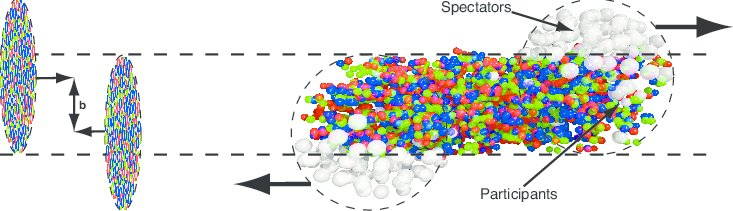
\includegraphics[width=0.99\linewidth]{Chapters/Introduction/Figs/collision.jpg}
\caption{Schematic of the stages on a heavy ion collision surrounding the collision moment. At first (left side) the nuclei are relativistically contracted. After the collision (right side) the spectators proceed unperturbed while the participants generate a colour tube filled of free partons.}
\label{fig:collision}
\end{center}
\end{figure}

The computed threshold can be crossed in ultra-relativistic heavy ion collisions
Such kind of collision involves a variable number of nucleons depending on the centrality of the collision.
The collision process is characterized by a complex space and time envelop, but can be divide in some macro-conditions which can help understanding the whole process \ref{fig:evolution}:
\begin{itemize}
    \item Before the collision the nuclei are Lorentz-contracted \ref{fig:collision}. The transverse spatial separation between the centroids of the two nuclei is called impact parameter and determines the number of nucleons participating to the interaction;
    \item at $t=0$ the collisions process starts and all the available energy is concentrated in the central region;
    \item Right after the collision the central "fireball" starts expanding following pressure gradients. The partons act as deconfined during this phase. The conservation of energy causes the temperature to drop depending on the fireball expansion;
    \item The chemical freeze-out happens when the average temperature drops below a threshold which at LHC amounts to $\simeq160 MeV$. The energy of the interactions does not allow to modify the abundances of hadrons;
    \item The thermal freeze-out corresponds to the moment in which the elastic interactions between hadrons stop.. At this point the kinematic spectra of the produced hadrons is fixed. The threshold temperature for this situation has be computed to be around $120 MeV$.
\end{itemize}

\begin{figure}[!t]
\begin{center}
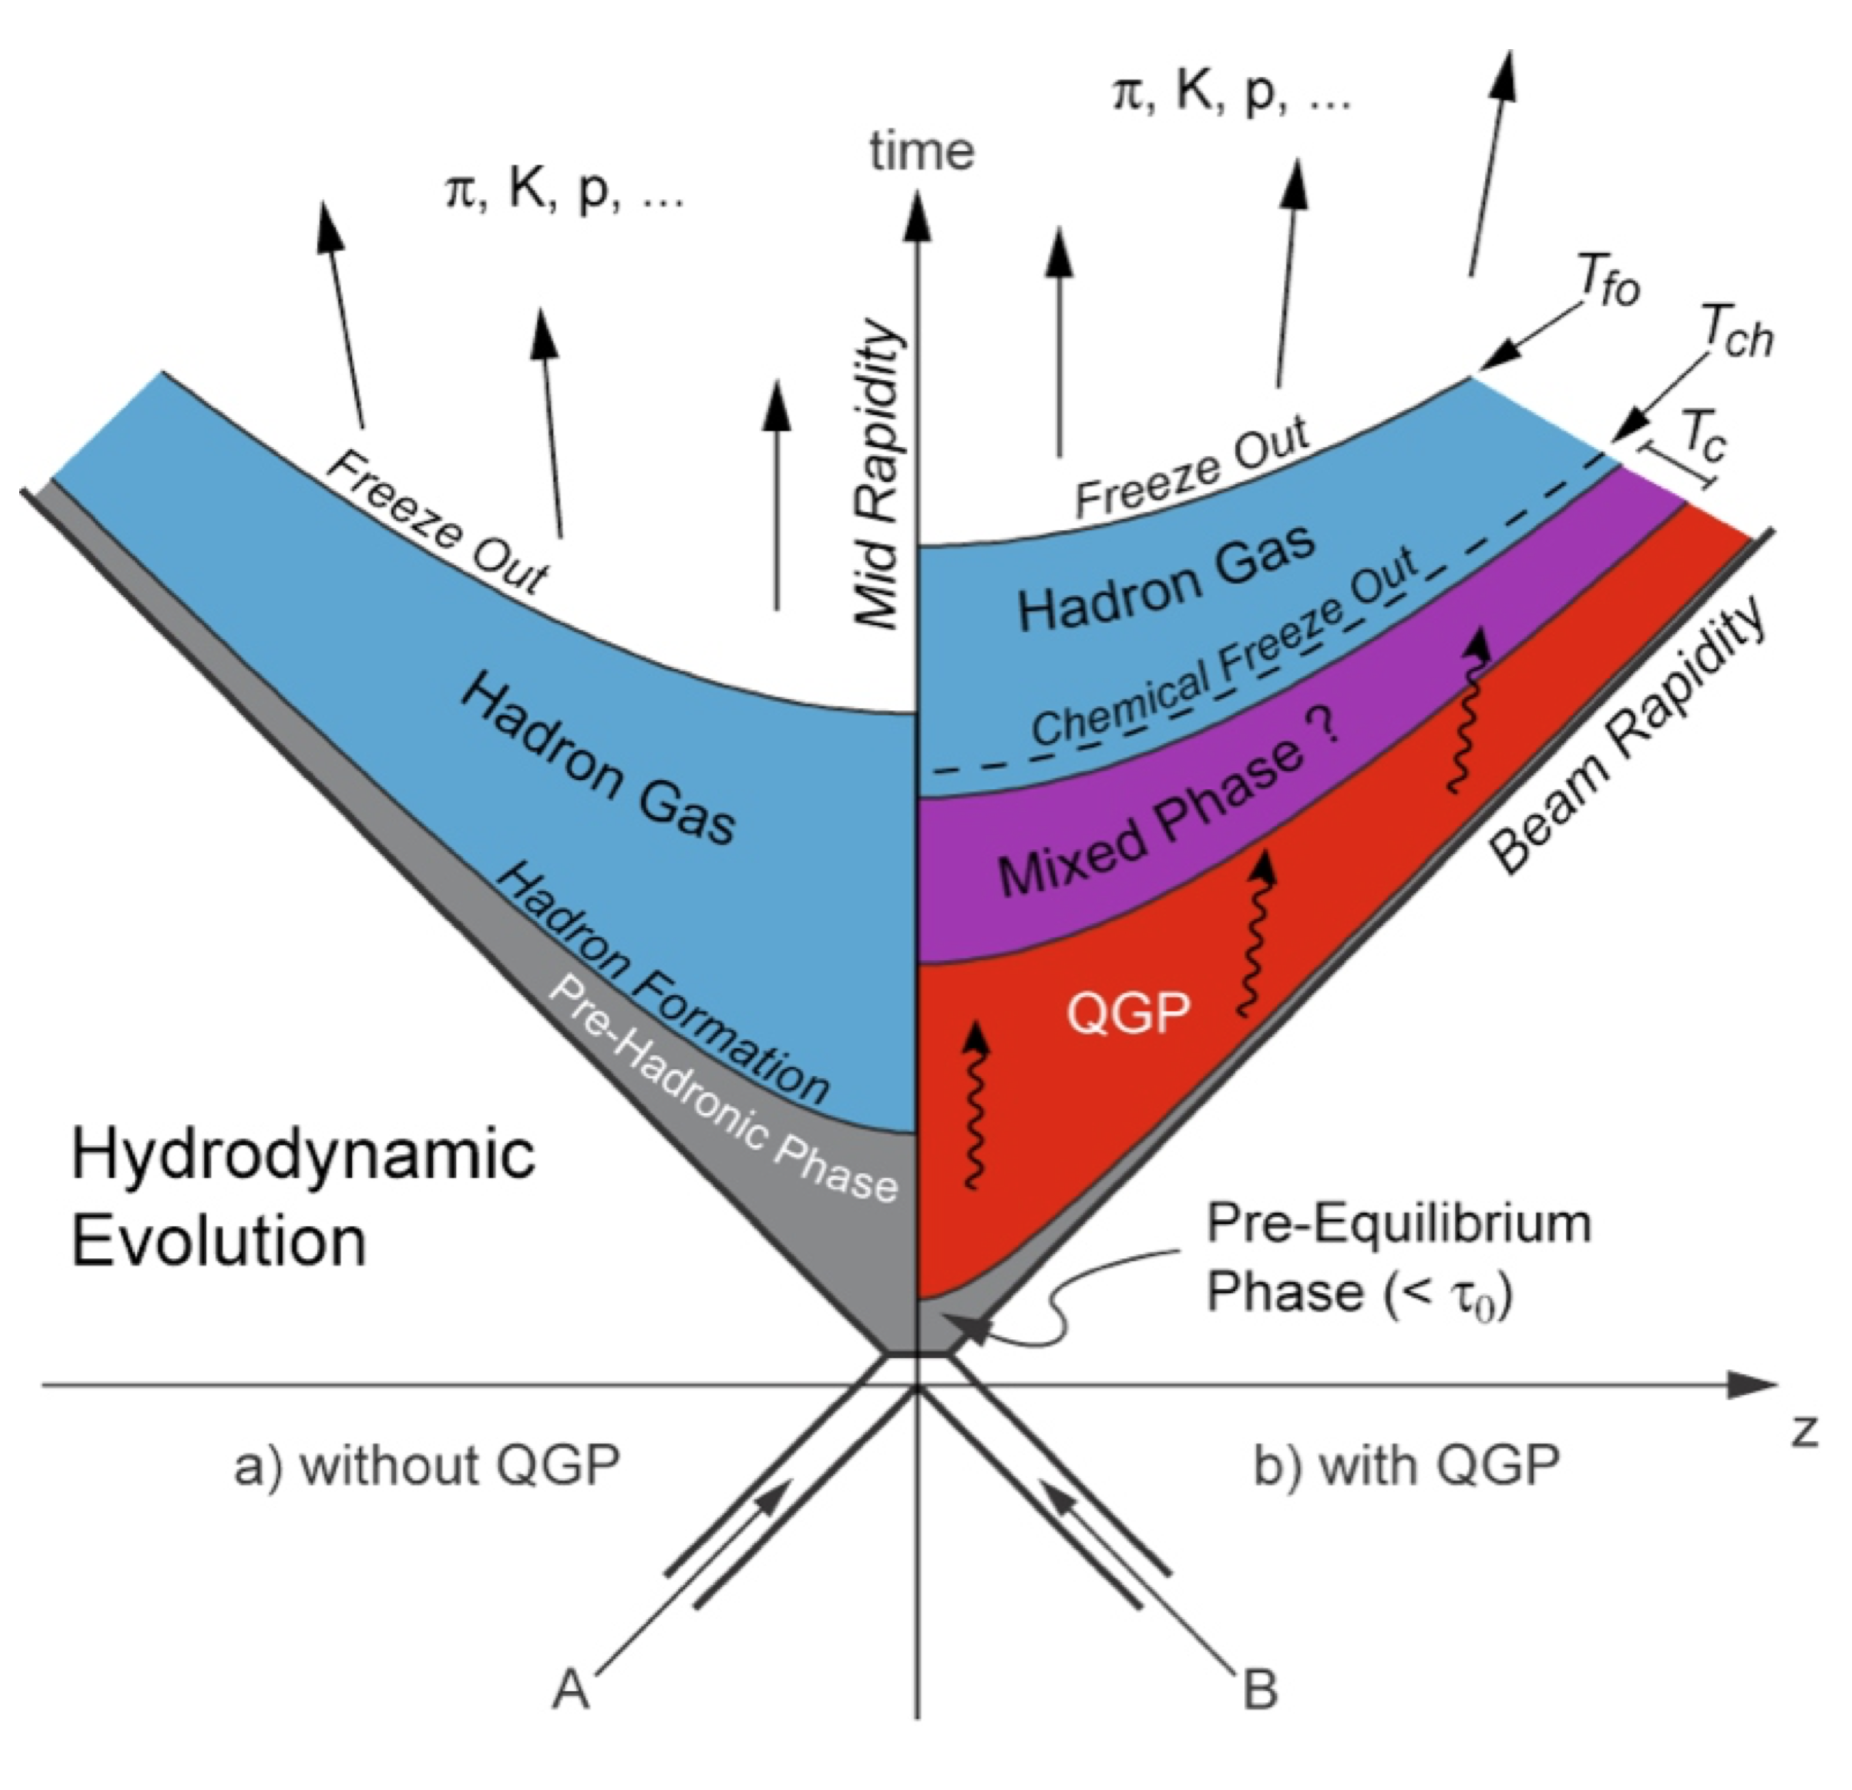
\includegraphics[width=0.85\linewidth]{Chapters/Introduction/Figs/QGP_evo.png}
\caption{Space-time evolution of the fireball originated from an heavy ion collision with (left) and without (right) QGP.}
\label{fig:evolution}
\end{center}
\end{figure}

The QGP phase is extremely short-lived and a direct observation is impossible.
However, after the thermal freeze-out the hadrons fly freely and they can be detected by the experiment.
This argument lead to the idea of studying the QGP by analyzing the emerging particles.
In fact emerging hadrons and particles which have been influenced by QGP formation, might bring some important information regarding its characteristics.

\subsection{Soft and hard probes}
The particles produced in a nuclear collision might be distinguished in soft and hard probes.
Soft probes are produced during the evolution of the system formed in the collision and are related to the collective behaviour of the medium.
The processes involving a soft probe production are characterized by low transferred momentum and for this reason $99.5\%$ of the produced particles are soft probes.
Some examples of soft probes are:
\begin{itemize}
    \item Particle multiplicity: the multiplicity of particles produced is important for the determi- nation of the energy density of the collision and the study of their transverse momentum spectra allows to obtain information on the chemical and thermal freeze-out;
    \item Collective flow: the spatial anisotropy of the colliding region induces pressure gradients which cause anisotropic particle distributions. This effect can be explained as a collective motion of particles produced in the interaction and its study is closely related to the determination of the equation of state for a deconfined medium;
    \item the study of these electromagnetic probes is important for the determination of the medium temperature.
\end{itemize}
By contrast to soft probes, hard probes are particles produced in high transferred momentum processes and they are characterized by much lower production cross section.
For this reason hard probes are produced early during the collision and can be strongly influenced by a deconfined medium.
Some examples of hard probes are:
\begin{itemize}
    \item Jet quenching: jets are produced by the fragmentation of high momentum partons. Inter- acting with a deconfined medium they can lose energy scattering with other free partons or through radiative gluon emission. The result is a quenched particle spectrum;
    \item heavy flavour multiplicity: states characterized by the presence of heavy quarks (charm or bottom) are very important in the study of QGP, especially via energy loss processes into a deconfined medium;
    \item Quarkonium production modification: the term quarkonium indicates a bound state of two heavy quarks and it is named charmonium when formed by charm quarks, bottomomium when formed by bottom quarks. These mesons are strongly affected by the formation of a partonic medium and this effect can result in a suppression due to a mechanism of color screening.
\end{itemize}

The bottomonium studied in the analysis chapter of this thesis belongs to the set of hard probes studied by ALICE.

\subsection{Centrality estimation: Glauber's model}\label{intro_glauber}
It is commonly known that nuclei are non poin-like objects.
Since each nucleon brings a part of the total nucleus momentum, the impact parameter of a nuclear collision determines the number of participant nucleons, hence the amount of available energy in the center of mass.
The measurement of the impact parameter is fundamental to know the nature of the initial collision state.
Glauber's model is the approximation usually used to model and analyze a nuclear collision characteristics, named after Roy Glauber.
The model stands on three basic assumptions:
\begin{itemize}
\item At high energy the nucleons are undeflected thanks to the large momentum, hence their trajectory is asymptotically linear;
\item Nuclear size has to be large compared to the range on nucleon-nucleon interaction;
\item Nucleons' motion independent from the nucleus one, hence the nuclear collision can be described in terms of the nucleon-nucleon cross section.
\end{itemize}

As one can already argue, the Glauber's approach to the description of nuclear collisions simplifies the problem diving to a more fundamental description, given at the nucleon level.
For doing so two inputs are necessary:
\begin{itemize}
\item Inelastic nucleon-nucleon cross section. 
This value should be measured at the same center-of-mass energy. 
It can be measured in proton-proton collisions;
\item Nucleus density profile. It is necessary to provide a contour shape for the colliding nuclei. 
Historically the nucleus profile has been modeled in the shell model approach as a Woods-Saxon distribution, which models the average nucleon potential in the nucleus. 
The potential shape corresponds to the nucleons distribution.
The Woods-Saxon distribution is represented in figure \ref{fig:WoodsSaxon} for a $Pb$ nucleus and presented in equation \ref{eq:WoodsSaxon}, where:
\begin{itemize}
\item $r$ is the radial position at which one wants to compute the nucleons density;
\item $\rho_0$ is the density value at $r=0$;
\item $\omega$ is a parameter which can represent a density bump right before the distribution tail;
\item $R$ is the radius at which $\rho/\rho_0=50\%$, similar to a half-width half maximum;
\item $a$ describes the steepness of the distribution's tail.
\end{itemize}
The Woods-Saxon distribution parameters are typically determined via $e^-$-nucleus scattering processes.
The differences between protons and neutrons are assumed to be negligible.

\begin{equation}
\label{eq:WoodsSaxon}
\rho(r) = \frac{\rho_0\cdot(1+\omega r^2/R^2)}{1+\exp(\frac{r-R}{a})}
\end{equation}

\end{itemize}

\begin{figure}[!t]
\begin{center}
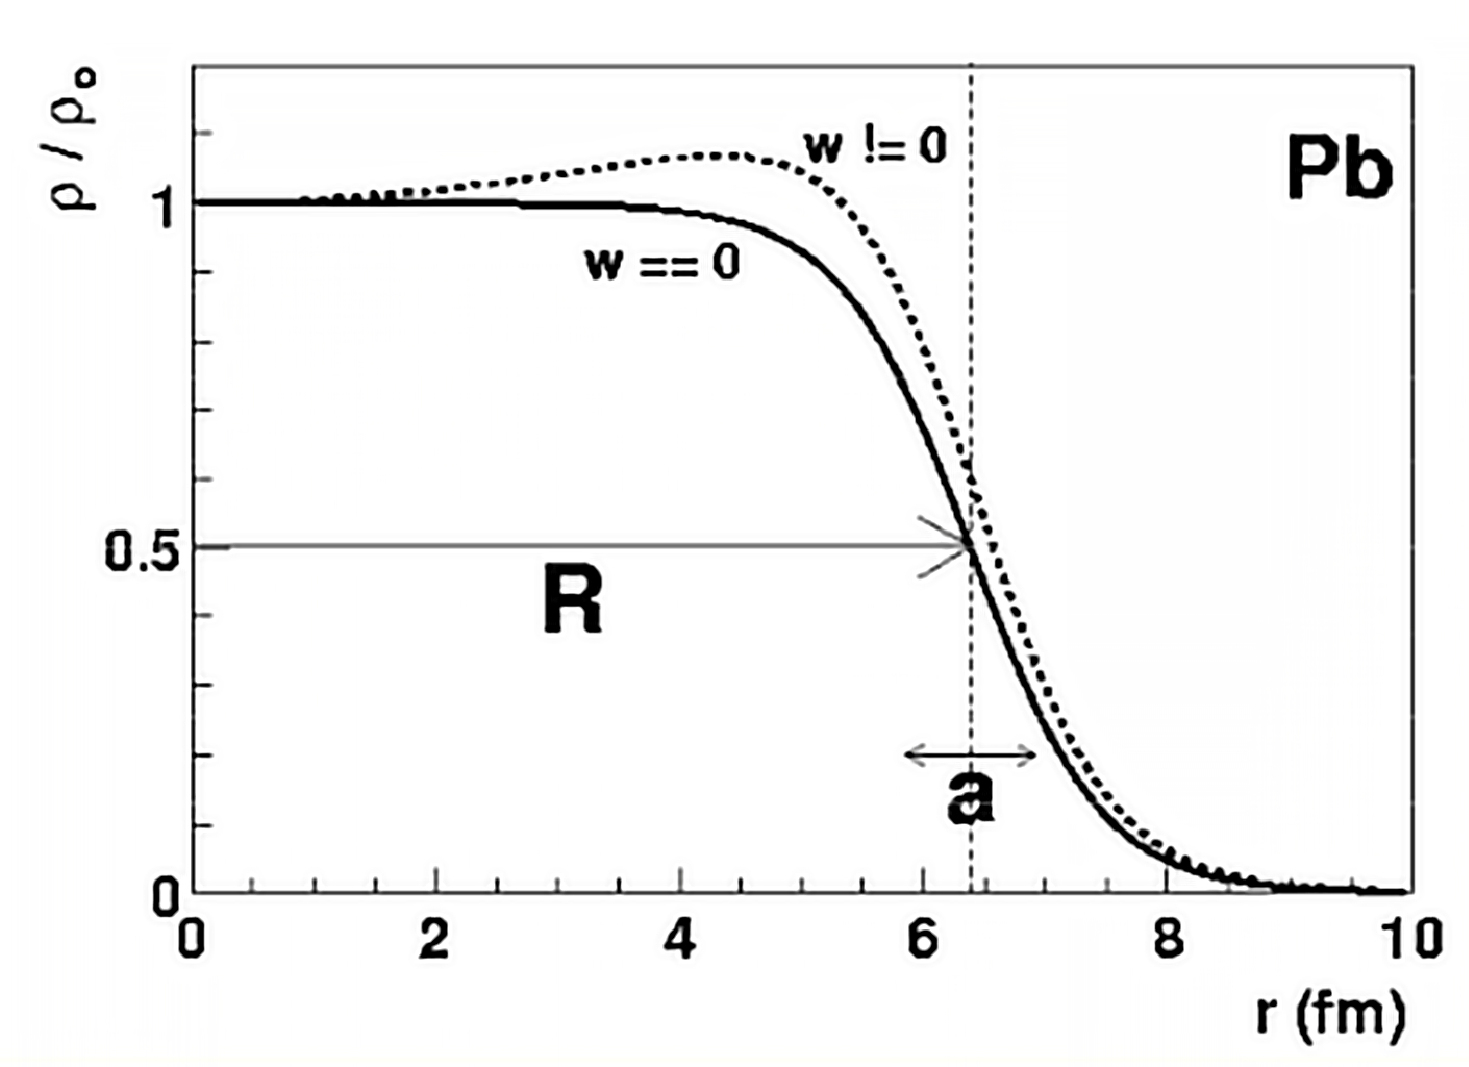
\includegraphics[width=0.7\linewidth]{Chapters/Analysis/Figs/woods-saxon.pdf}
\caption{Woods-Saxon potential for $Pb$ nucleus as the ration of the $\rho(r)$ over $\rho_0$ as a function of the distance from the nucleus center ($r$).
Displayed parameters are extensively described in paragraph \ref{intro_glauber}}
\label{fig:WoodsSaxon}
\end{center}
\end{figure}

\begin{figure}[!t]
\begin{center}
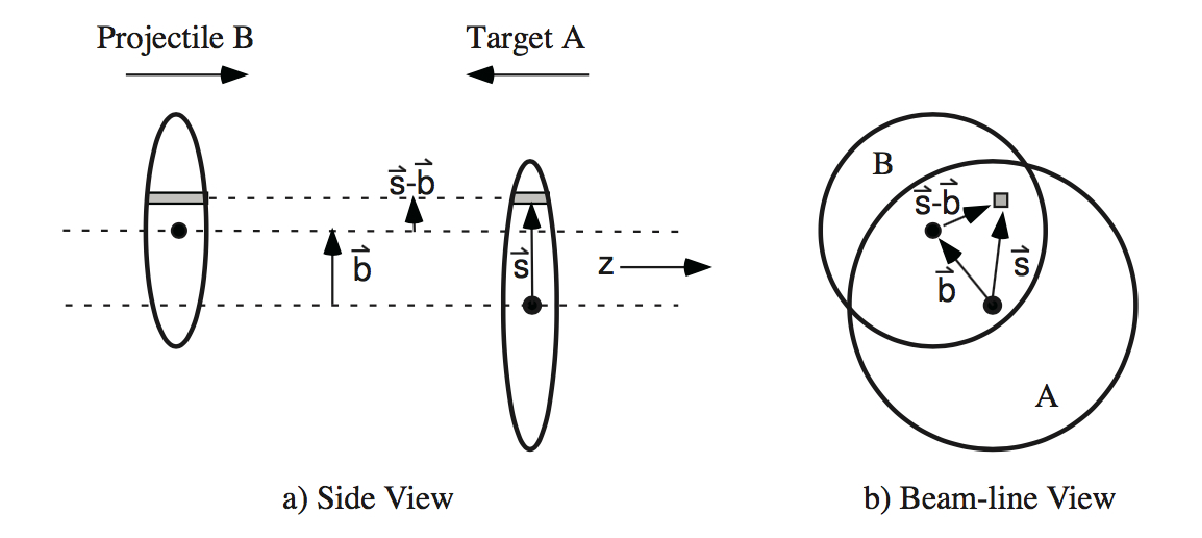
\includegraphics[width=0.85\linewidth]{Chapters/Analysis/Figs/glauber-side.pdf}
\caption{Schematic representation of the Optical Glauber Model geometry, with transverse (a) and longitudinal (b) views. From \cite{Miller:2007ri}.}
\label{fig:GlauberSide}
\end{center}
\end{figure}

The Glauber's model uses an optical and geometric approach to represent the nuclear collision.
Referring to picture \ref{fig:GlauberSide}:
\begin{itemize}
\item $b$ is the distance between the centers of the colliding nuclei, namely the impact parameter;
\item $s$ is the distance of a nucleon flux tube relative to the nucleus center.
\end{itemize}
Note that in this discussion the vectors $\vec{b}$ and $\vec{s}$ will be replaced by their modulus.
This can be done if the colliding particles are not polarized and present a spherical distribution of probability for the nucleon density.
This assumption is legitimate for Pb nuclei.

The probability of finding a nucleon in a nucleon flux tube posed at $s$ from target A is defined in equation \ref{eq:TAs}.
The same equation can be rephrased to compute the same probability for the projectile, namely B.

\begin{equation}
\label{eq:TAs}
\hat{T}_A(s) = \int\hat{\rho}_A(s,z_A)dz_a
\end{equation}

The effective overlap area of two specific nucleons can be described by the equation \ref{eq:TAB}, in which the definition introduced in \ref{eq:TAs} is extensively adopted.
$\hat{T}_{AB}(\vec{b})$ dimension is an inverse area.

\begin{equation}
\label{eq:TAB}
\hat{T}_{AB}(b) = \int\hat{T}_A(s)\hat{T}_B(s-b)d^2s
\end{equation}

The probability of inelastic interaction between two specific nucleons belonging to A and B respectively can be described by equation \ref{eq:PAB}.

\begin{equation}
\label{eq:PAB}
P_{AB}(b)=\hat{T}_{AB}(b)\sigma_{inel}^{NN}
\end{equation}

Since the nucleons in A and B are not distinguishable, this interaction probability has to be reworked in order to loose the attribute of being specific for two nucleons.
Using a binomial distribution of probability one obtains \ref{eq:Pnb}, where $AB$ is the product of the number of nucleons and $n$ in the number of desired nucleon-nucleon collisions.

\begin{equation}
\label{eq:Pnb}
P(n,b)=\binom{AB}{n}[P_{AB}(b)]^n[1-P_{AB}(b)]^{AB-n}
\end{equation}

Using the last equation, defining:
\begin{itemize}
\item Collision: a nucleon-nucleon collision;
\item Participant: a nucleon which takes part to at least one nucleon-nucleon collision;
\item Spectator: a nucleon which doesn't take part to any collision.
\end{itemize}
one can compute $N_{coll}(\vec{b})$ (number of nucleon-nucleon collisions), $N_{part}(\vec{b})$ (number of participant nucleons) and $N_{spec}(\vec{b})$ (number of spectator nucleons).

\begin{equation}
\label{eq:Ncoll}
N_{coll}(b)=\sum_{n=1}^{AB}nP(n,b)=AB\hat{T}_{AB}(b)P_{AB}(b)
\end{equation}

\begin{equation}
\label{eq:Npart}
N_{part}(b)=A\int\hat{T}_A(s){1-[1-P_{AB}(s-b)]}d^2s + B\int\hat{T}_A(s-b){1-[1-P_{AB}(s)]}d^2s
\end{equation}

\begin{equation}
\label{eq:Nspec}
N_{spec}(b)=A+B-N_{part}(b)
\end{equation}

In figure \ref{fig:GlauberAuAu} participants of a $Au--Au$ collision are shown in strong blue and red, while semi-transparent blue and red dots represent the spectators.

\begin{figure}[!t]
\begin{center}
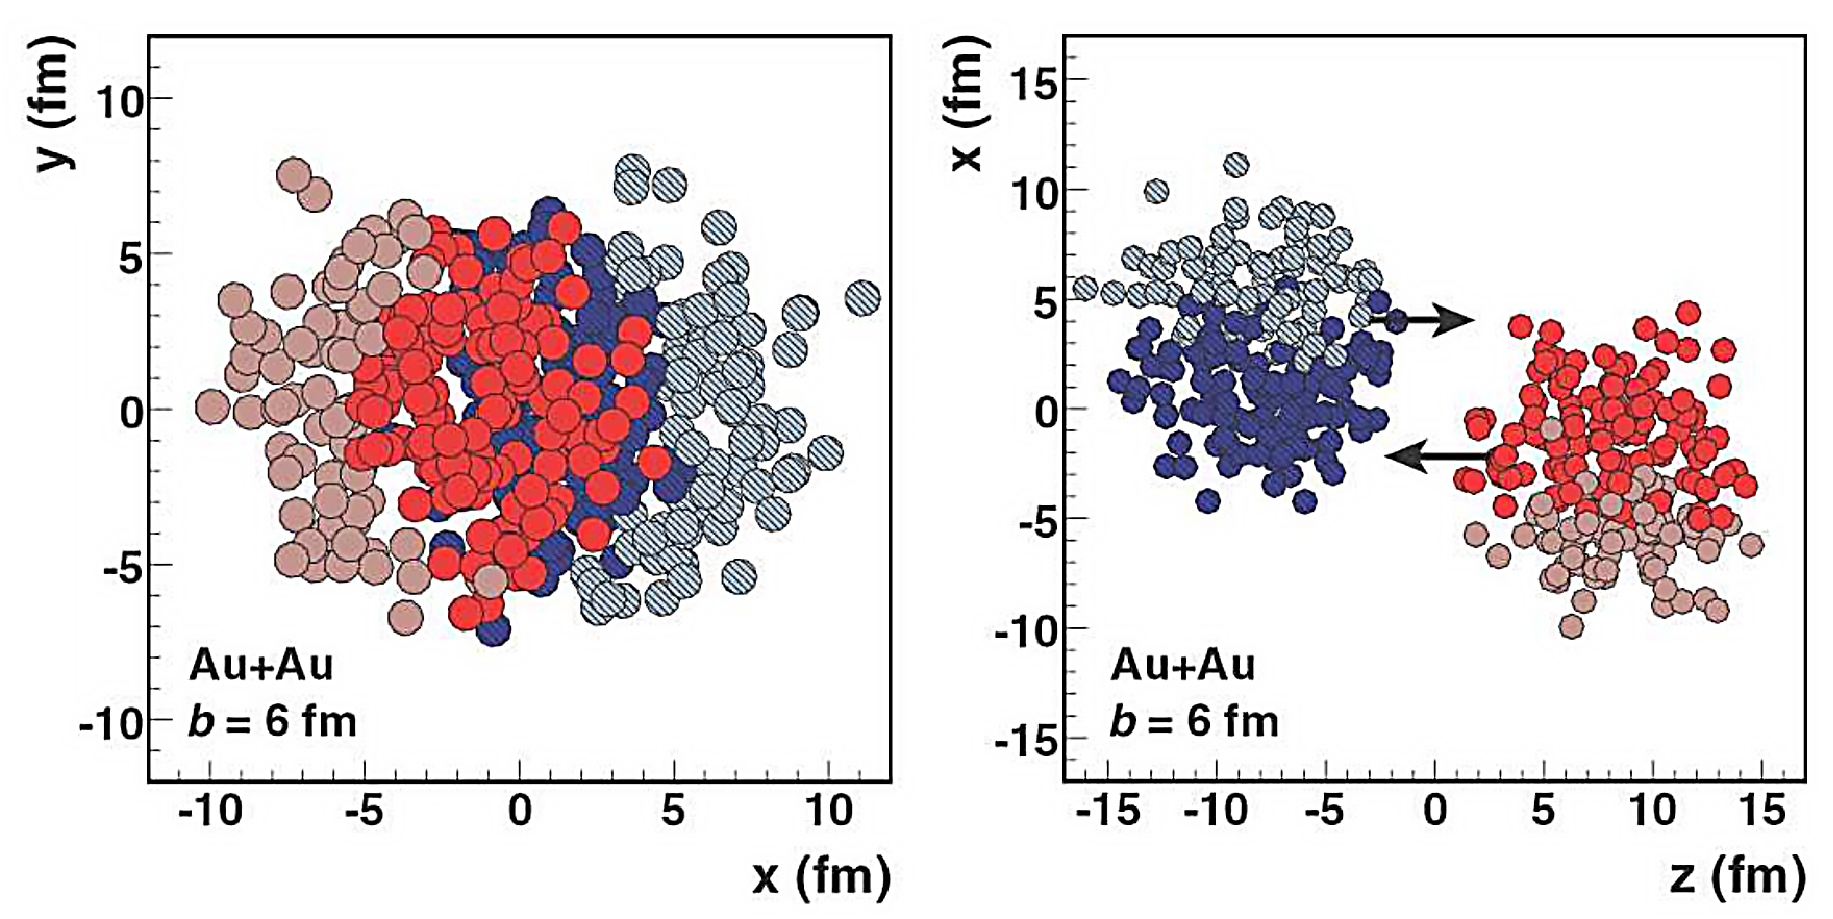
\includegraphics[width=0.9\linewidth]{Chapters/Analysis/Figs/glauber-pbpb.pdf}
\caption{Glauber Monte Carlo $Au--Au$ collision with impact parameter $b=6 fm$ seen in the trasverse plane (left) and along the beam axis (right). Nucleons area is equal to $\sigma_{inel}^{NN}$. From \cite{Miller:2007ri}.}
\label{fig:GlauberAuAu}
\end{center}
\end{figure}

Through the Glauber's model a measurement of the number of participant or spectator nucleons can provide an indirect measurement of the impact parameter of a nuclear collision.
Unfortunately neither $N_{part}(b)$ nor $N_{spec}(b)$ can be directly measured.
Typically the number of participants is related to the charged particles multiplicity ($N_{ch}$).
$N_{ch}$ has been measured over a large range of rapidity and is well described by a negative binomial distribution \cite{Aamodt:2009aa}.
This approach allows to simulate an experimental multiplicity distribution that can then be linked to an experimental observable.
In figure \ref{fig:GlauberCent} the collision probability is represented as a function of $N_{ch}$. Additional axes represent the correlation between centrality and $N_{part}$, $b$ and fraction of the total cross section $\sigma/\sigma_{tot}$.
For ALICE one of the detectors, the VZERO, provides a signal whose amplitude is the $N_{ch}$ estimation provider, hence the source of the main centrality evaluation, as shown in picture \ref{fig:GlauberVZERO}.


\begin{figure}[!t]
\begin{center}
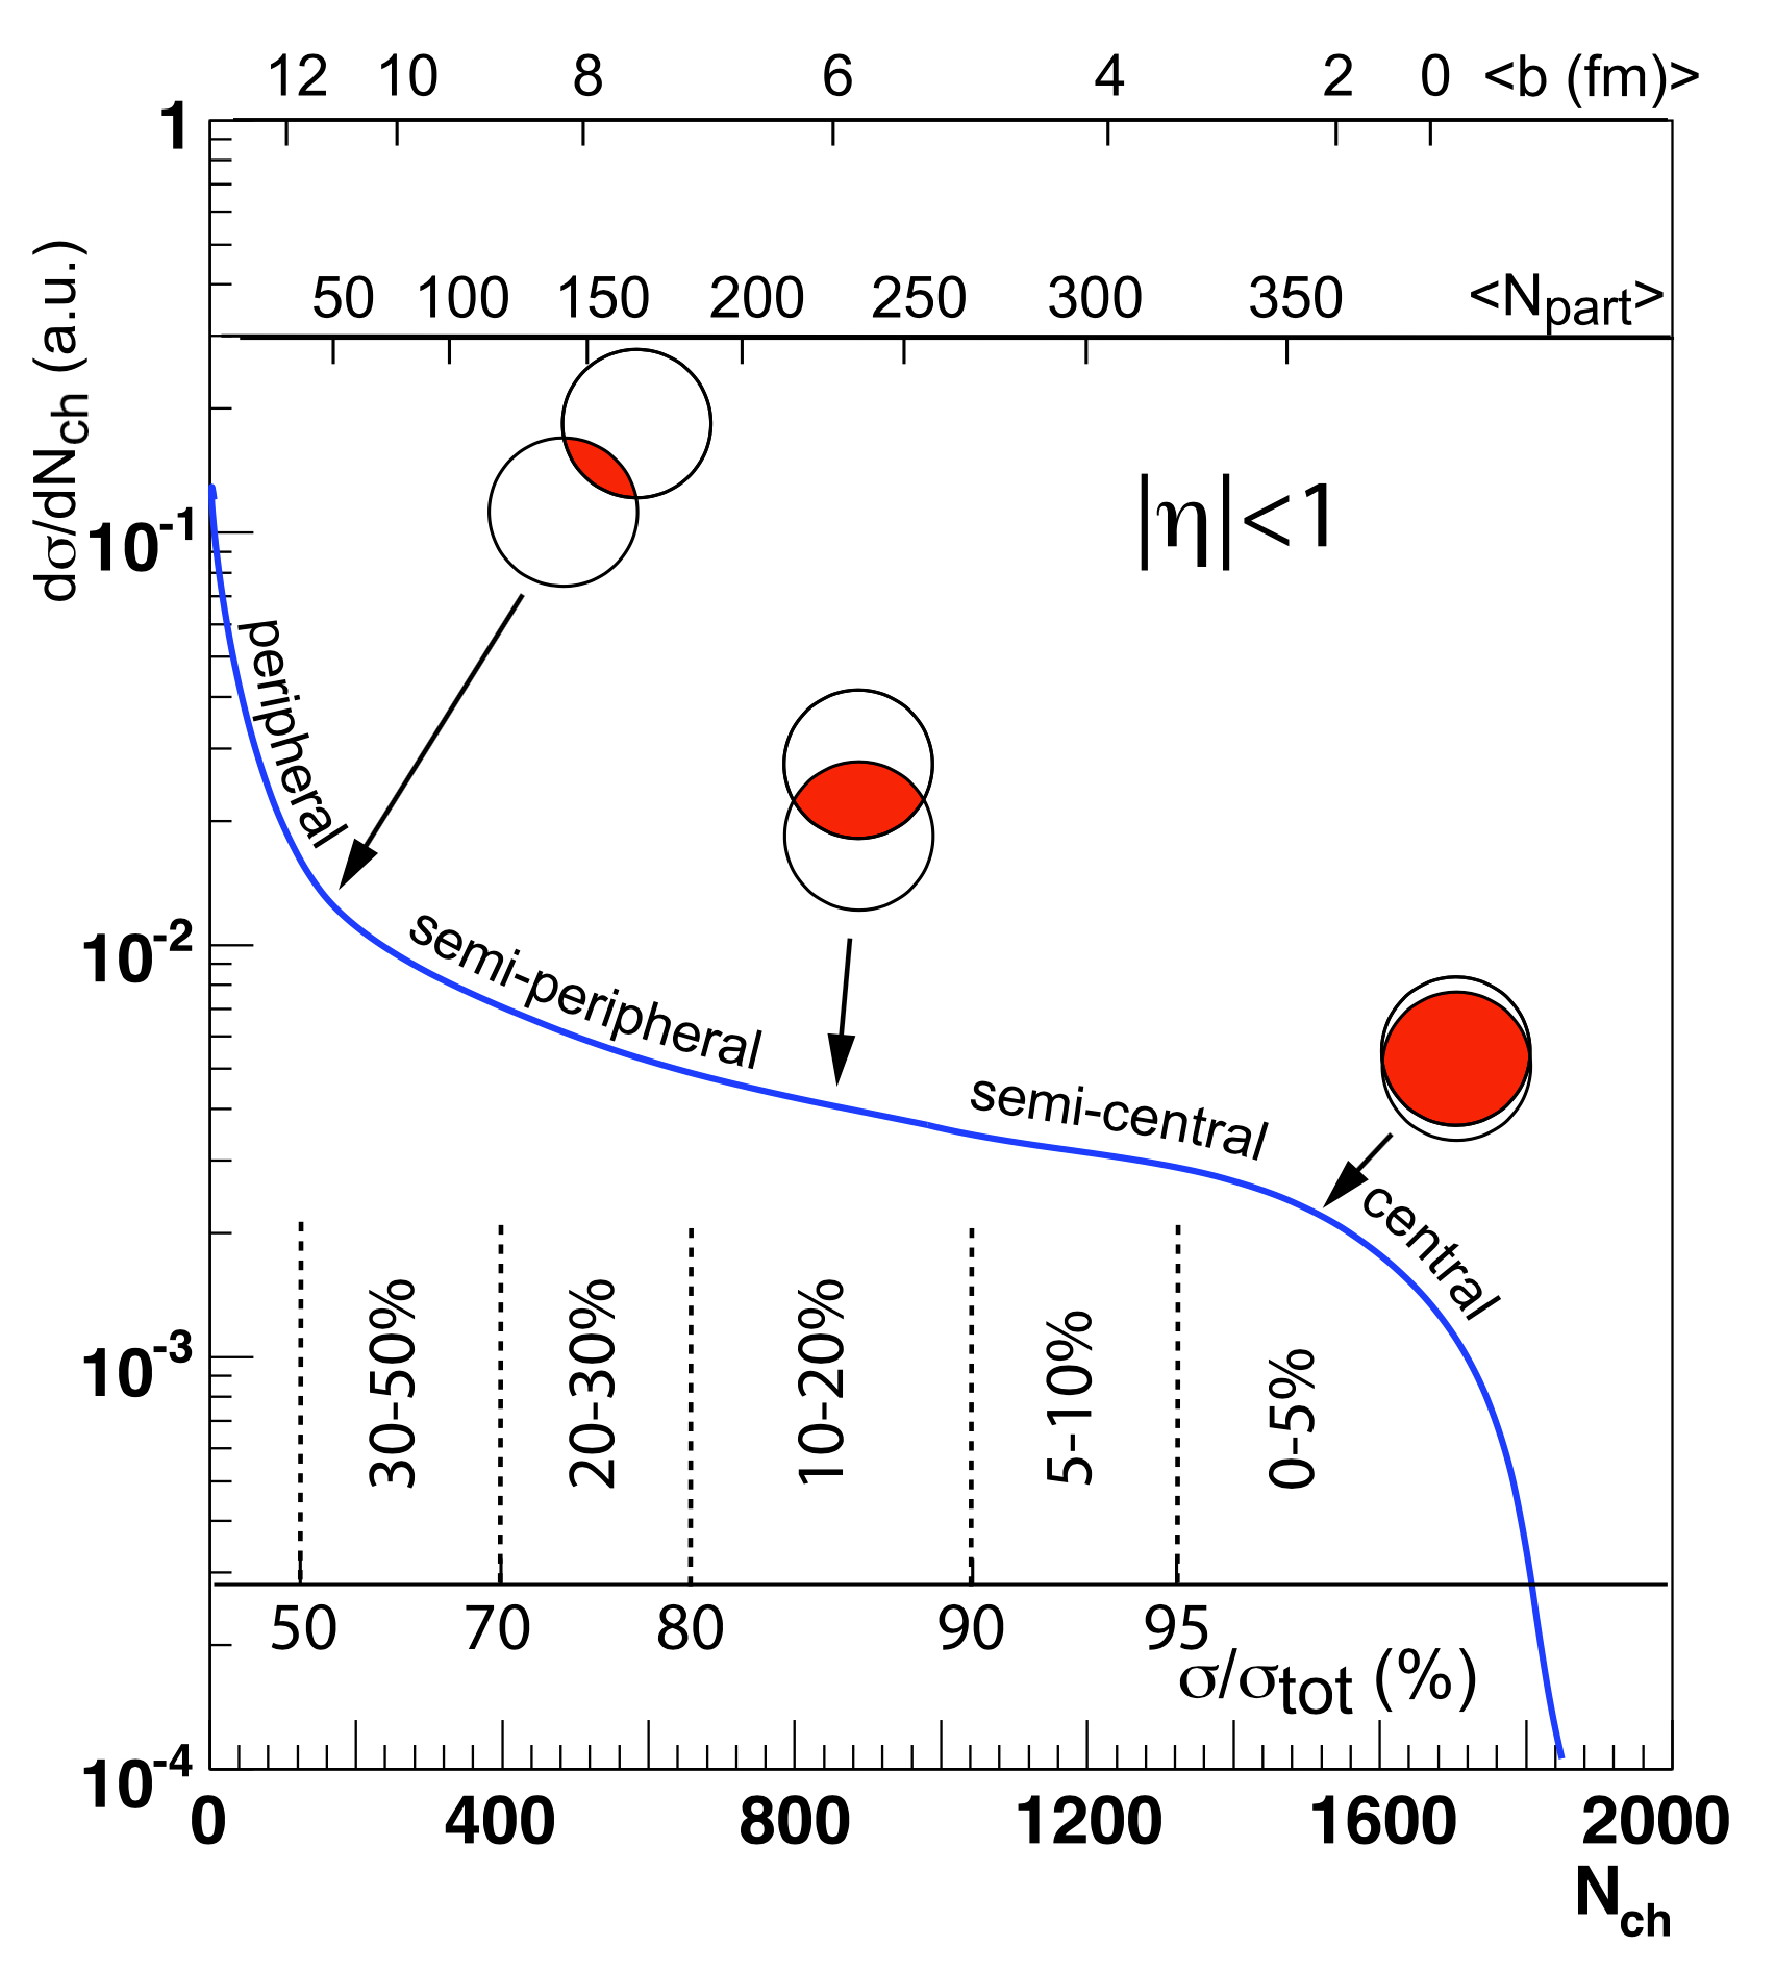
\includegraphics[width=0.75\linewidth]{Chapters/Analysis/Figs/glauber-centrality.pdf}
\caption{A cartoon example of the correlation of the final state observable $N_{ch}$ with Glauber calculated quantities ($b$, $N_{part}$). The plotted distribution and various values are illustrative and not actual measurements. From \cite{Miller:2007ri}.}
\label{fig:GlauberCent}
\end{center}
\end{figure}

\begin{figure}[!t]
\begin{center}
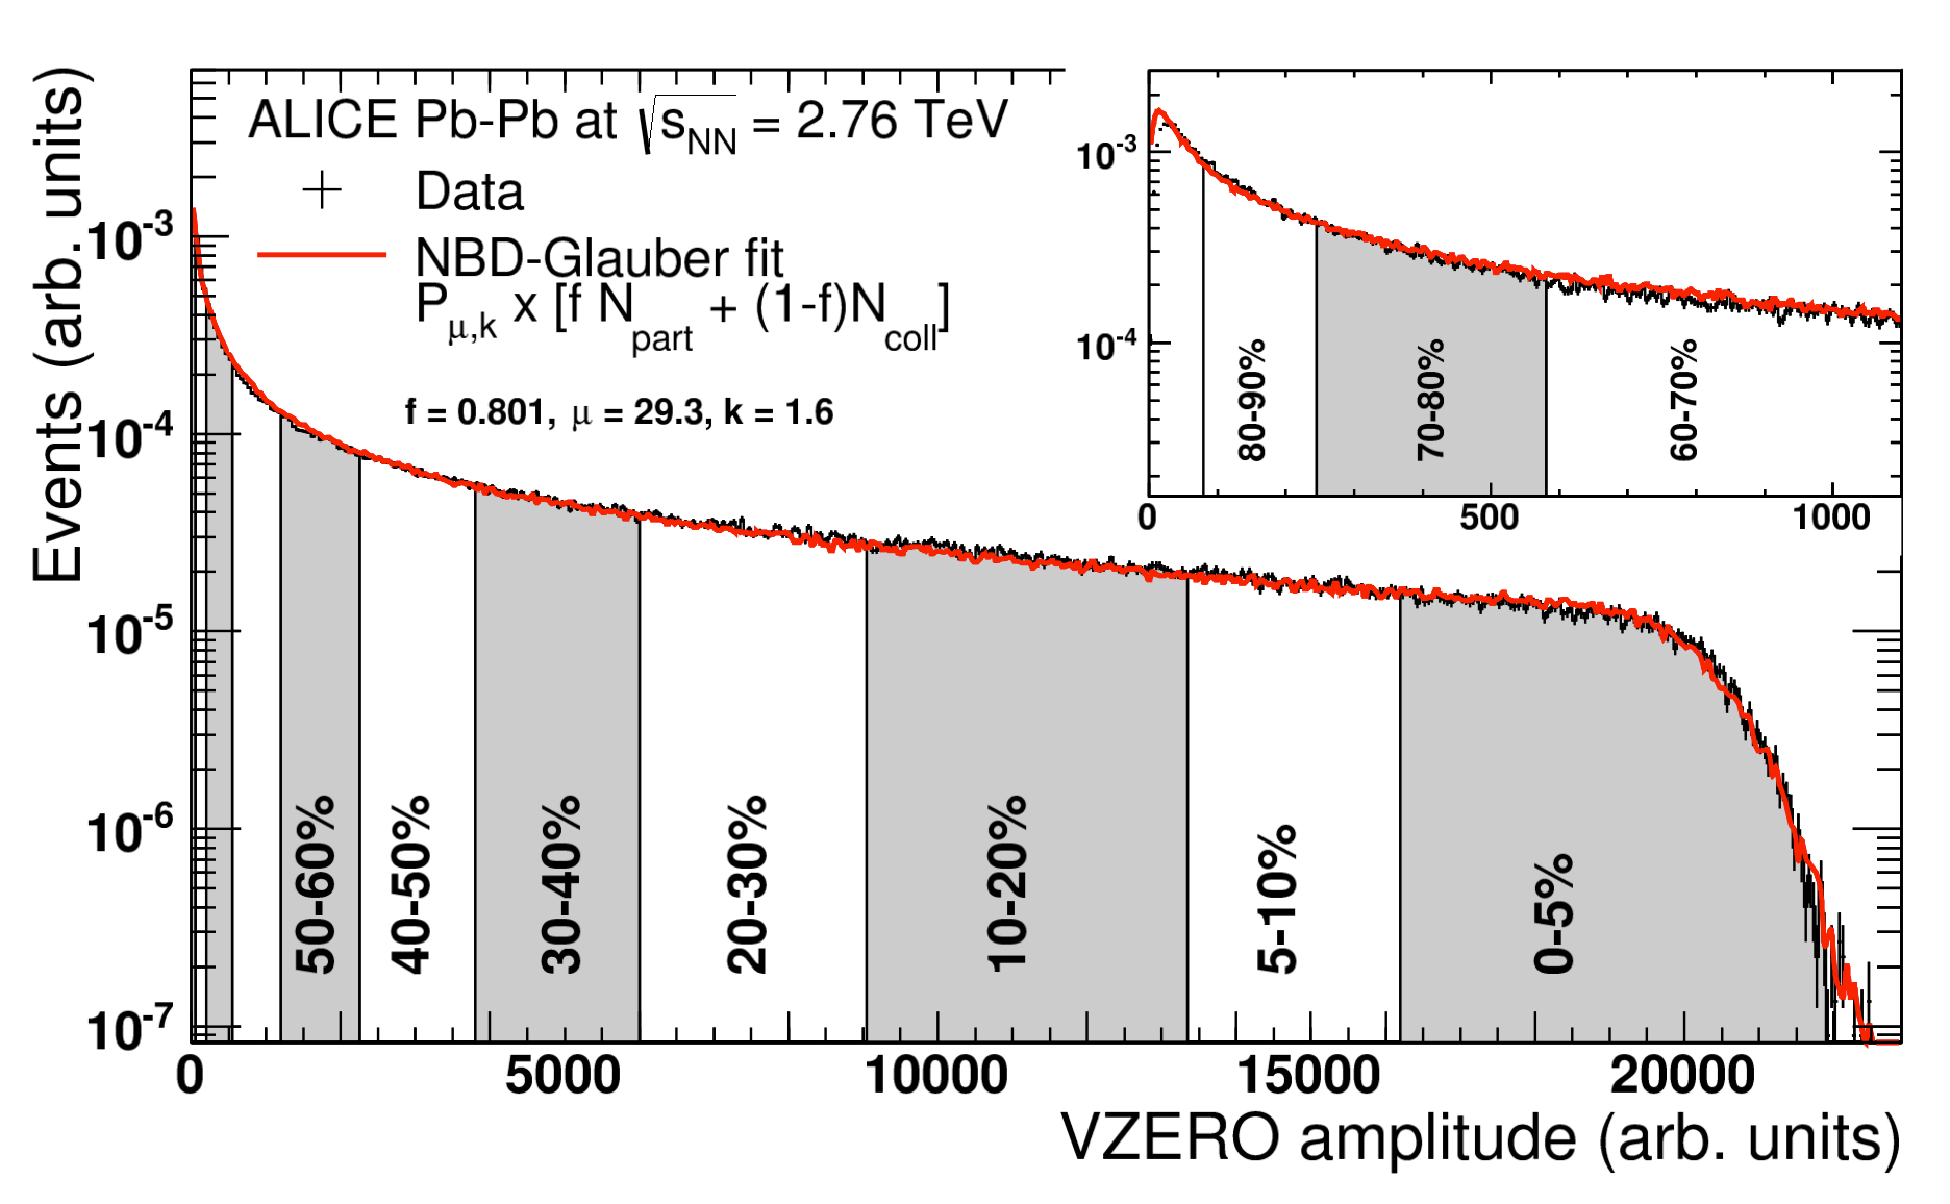
\includegraphics[width=0.85\linewidth]{Chapters/Analysis/Figs/glauber-vzero.pdf}
\caption{Distribution of the sum of amplitudes in the VZERO scintillators. The distribution is fitted with the NBD-Glauber fit shown as a red line. The centrality classes used in the analysis are indicated in the figure. The inset shows a zoom of the most peripheral region. From \cite{Abelev:2013qoq}.}
\label{fig:GlauberVZERO}
\end{center}
\end{figure}

\subsection{Nuclear modification factor}\label{RAA}
In general the study of the modifications of the production of probes in heavy nuclei collisions, with respect to proton--proton collisions, makes use of the nuclear modification factor definition.
The definition of the nuclear modification factor follows the Glauber's approach, using its model observables to obtain a centrality-dependent form.
The simplest mathematical form of the nuclear modification factor is the one reported in \ref{eq:RAA}.

\begin{equation}[!t]
\label{eq:RAA}
R_{\rm{AA}}^X = \frac{N_{\rm{AA}}^X}{<N_{coll}>\cdot N_{\rm{pp}}^X}
\end{equation}

Where $R_{\rm{AA}}^X$ is the nuclear modification factor for the species $X$, $<N_{coll}>$ is the number of binary nucleon--nucleon collisions happening in the nucleus--nucleus collision and $N_{\rm{(pp,AA)}}^X$ are the yields of $X$ states in a proton--proton and a nucleus--nucleus collision, respectively.
The formulation of the denominator of the fraction defining the $R_{\rm{AA}}^X$ originates from the assumption that nucleons in a nucleus behave as an incoherent superposition of $A$ nucleons.
To simplify, the denominator corresponds to the number of $X$s one would be able to measure in the case in which the binding between nucleons in the nuclei would have no effect on the single binary collision.
Moreover the denominator formulation models that during each binary collision the spectator nucleons are neither participating nor perturbing the binary collision outcome.
The meaning of $R_{\rm{AA}}^X$ is then trivial: it represents the deviation from the "ideal" situation in which mutual interactions between nucleons have no visible effect of the yields of a nucleus--nucleus collision.

\begin{equation}
\label{eq:yields}
N_{\rm{pp}}^X = \frac{\sigma_{\rm{pp}^{X}}}{\sigma_{\rm{pp}_{MB}}}
\end{equation}

The yields of a given state $X$ can be defined using its cross-section. The definition reported in \ref{eq:yields} can be then introduced in \ref{eq:RAA} giving a definition of the nuclear modification factor which is more suitable for substitution with measurements. This substitution can be rewritten using the Glauber's model definition of nuclear overlap factor as in equation \ref{eq:TAA}, leading to \ref{eq:RAA2}.

\begin{equation}
\label{eq:TAA}
T_{\rm{AA}} = \frac{<N_{coll}>}{\sigma_{\rm{pp}_{MB}}}
\end{equation}

\begin{equation}
\label{eq:RAA2}
R_{\rm{AA}}^X = \frac{N_{\rm{AA}}^X}{T_{\rm{AA}} \cdot \sigma_{\rm{pp}}^X}
\end{equation}

For the nuclear modification factor three scenarios can be foreseen for the nuclear modification factor values:
\begin{itemize}
\item $R_{\rm{AA}}^X<1$: a nucleus--nucleus collision presents a net suppression of the production of $X$s;
\item $R_{\rm{AA}}^X>1$: during the nucleus--nucleus collision a net enhancement of the production of $X$s is observed; 
\item $R_{\rm{AA}}^X=1$: the nucleus--nucleus collision can be interpreted as an incoherent superposition of binary nucleon--nucleon collisions. Note that this situation might occur even in the case where suppression and enhancement effects balance out perfectly.
\end{itemize}

\section{Bottomonium study}
\subsection{Rationale of bottomonium study} %Section - 3.1
A detailed study of the properties of the Quark-Gluon Plasma (QGP)~\cite{Shuryak:1978ij} is the main goal of heavy-ion experiments at ultra-relativistic energies~\cite{Adams:2005dq,Muller:2012zq}.
ALICE joins the efforts of the previous generation of similar experiments, extending the reach of such studies.

Quarkonia, $i.e.$ bound states of charm or bottom quark-antiquark pairs, are sensitive probes of color deconfinement, due to the QCD Debye screening mechanism  \cite{Matsui:1986dk,Brambilla:2010cs,Andronic:2015wma}. 
Due to their heavy mass, heavy quarks are produced in the initial parton--parton interactions.
While propagating in the hot and dense medium they experience the full evolution of the QGP. 
In addition, the quarkonium states binding energies may greatly differ from one state to another.
Thinking about a dissociation process \textit{à la Debye}, the different binding energies imply different dissociation temperatures in a QGP.
This peculiarity leads to a sequential suppression of differently bound states ~\cite{Digal:2001ue}. 
In such scenario, the lighter the quarkonia states are bound, the more likely they happen to be melt by the QGP.
If this dissociation process happens only part of the total production of a given quarkonium state will emerge from the QGP region.

First studies of quarkonium production in heavy-ion collisions were devoted to charmonium states, and a suppression of their yields was observed
at the SPS~\cite{abreu:in2p3-00002434,Alessandro:2004ap,Arnaldi:2007zz}, at RHIC~\cite{Adare:2011yf,Abelev:2009qaa} and at the LHC~\cite{Abelev:2012rv,Chatrchyan:2012np,Adam:2016rdg}. 
The much weaker \jpsi suppression observed at LHC energies, despite the centre-of-mass energy per nucleon pair (\snn) being one order of magnitude larger than at RHIC, is now explained by means of a competition between suppression and regeneration phenomena, which occurs during the deconfined phase and/or at the hadronization stage of the system~\cite{BraunMunzinger:2000px,Thews:2000rj,Zhao:2011cv,Zhou:2014kka}.
In general free quarks and anti-quarks of the same species may form a quarkonium bound state.
At the LHC energies, the high abundance of charm and bottom quarks  makes not-negligible the probability of the regeneration to occur.
While at RHIC the charm pairs abundance was of about $10$ pairs per central collision, at the LHC the estimation rises to $\approx 100$.
The recombination process can lead to an enhancement of the production of a given quarkonium state, providing a concurrent effect to the aforementioned suppression and has been found to be more important at low $p_{\rm T}$(due to easier recombination at low $p$) and in the most central collisions (due to higher parton density) \cite{Abelev:2013ila,Adam:2015isa}.

The separation of suppression and regeneration mechanisms' effects is a puzzling task.
Models able to reproduce the charmonium states production rates include a regeneration contribution.
The abundances of charm and anti-charm quarks, at the LHC collision conditions, make the regeneration contribution important.
Decoupling of the concurrent effects using measurements on the charmonium states appears to be not trivial.
Is however worth mentioning that bottom quarks pairs abundance at the LHC is expected to be similar to the charm pairs abundance at RHIC, hence the recombination effect should be negligible for the bottomonium states.
Bottomonium states are expected to be much less affected by recombination with respect to charmonium states, due to the higher mass of the bottom quarks, hence to their lower abundance.
Since the  ${\rm b{\overline b}}$ yield in central heavy-ion collisions amount to a few pairs ($\approx 10$) per event at the LHC, the probability for regeneration of bottomonia through recombination is much smaller than in the case of charmonia ($\approx 100$ pairs).
The much lower regeneration contribution makes the bottomonium states the best candidates for a Debye-based QGP thermometer \ref{fig:QGP_thermo}.

\begin{figure}[!t]
\begin{center}
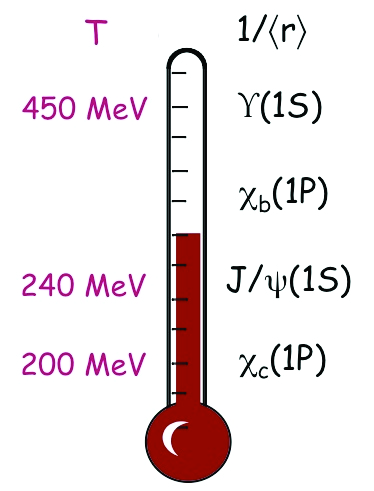
\includegraphics[width=0.3\linewidth]{Chapters/Analysis/Figs/QGP_thermometer.png}
\caption{Representation of a dissociation based QGP thermometer. The suppression of energetically ordered resonances can provide informations regarding the average kinetic energy of the formed QGP droplet.}
\label{fig:QGP_thermo}
\end{center}
\end{figure}

Is worth mentioning that, for bottomonium production, perturbative calculations of production rates in elementary nucleon-nucleon collisions are more reliable than for charmonium yields due to the higher mass of the bottom quark with respect to charm. 

In conclusion the study of bottomonium production can provide an independent measurement of QGP characteristics, adding up to charmonium measurements to better understand the dissociation and recombination contributions to quarkonia production.

\subsection{Complexity of bottomonium study}
Due to the higher mass of the constituting quarks, the abundance of bottomonium states in the final state of QGP evolution is much lower if compared to those of charmonium states.
This physical characteristic limits the available statistics.
In addition bottomonium production theoretical estimates \cite{Krouppa:2015yoa} indicate that its formation may occur before QGP thermalization \cite{Mauricio:2007vz}. 
In this situation, a quantitative description of the influence of the medium on the bound states becomes challenging.
Even if the dissociation temperatures may vary significantly between different models \cite{Brambilla:2010cs,Andronic:2015wma}, it is commonly accepted \cite{Burnier:2014ssa} that the spectral functions of the bottomonium states are affected by the high temperature of the surrounding medium.
This effect leads to much larger spectral widths than in vacuum.
Finally, even if the regeneration of bottomonium can be considered negligible at LHC energies, another production enhancement effect partly disrupts the possibility to use bottomonium states as a QGP thermometer. 
In fact, taking into account that feed-down processes from higher-mass resonances  are not negligible (around 40\% for the \upsis and 30\% for the \upsiss \cite{Andronic:2015wma}), the evaluation of the medium temperature via bottomonium measurements remains a complex endeavour.

\begin{figure}[!t]
\begin{center}
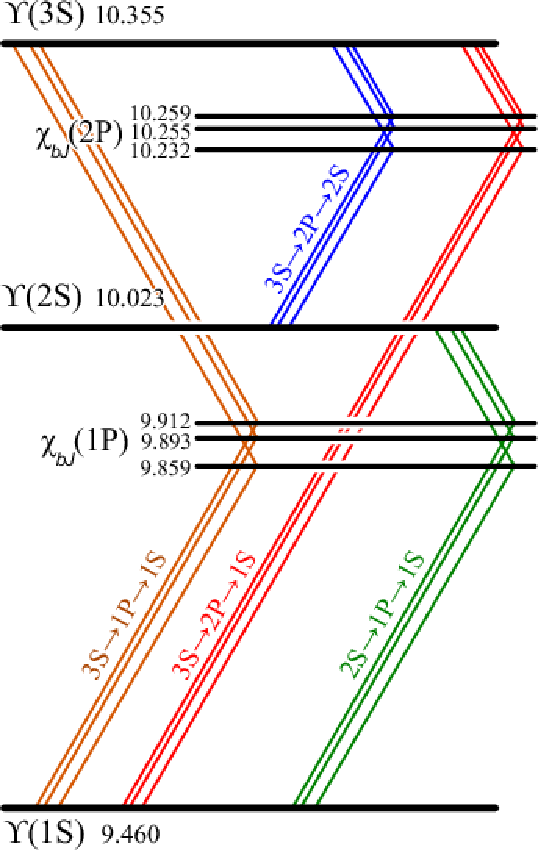
\includegraphics[width=0.45\linewidth]{Chapters/Analysis/Figs/BottomoniumSpectro.pdf}
\caption{Representation of possible feed-down patterns for bottomonium states as measured from BaBar collaboration and reported in \cite{Lees:2014qea}. The numbers refer to the masses as reported by the PDG. Each cascade terminates with the annihilation $\Upsilon(nS)\Rightarrow\mu^+\mu^-$, not shown. Splittings in the photon spectra for these cascades are due to the mass splittings in the intermediate states $\chi_{bJ}$ with J = 0, 1 or 2.}
\label{fig:BBSpectro}
\end{center}
\end{figure}

\subsection{Previous results}
Before the operations of LHC, the RHIC accelerator was leading the edge of QGP-oriented research.
The PHENIX collaboration measured the $J/\psi$ suppression in Au-Au collisions at $\sqrt{s_{_{\rm NN}}}=200$ GeV, highlighting a suppression strongly correlated with the centrality of the collision.
Given the much lower available energy at RHIC, with respect to the LHC, the recombination effects were not visible, yet unexpected.
The first $J/\psi$ measurements at the LHC disrupted the commonly accepted models, since, despite expectations, a much lower $J/\psi$ suppression was observed in the most central collisions at LHC at $\sqrt{s_{_{\rm NN}}}=2.76$ \rm{TeV} with respect to what had been observed at $\sqrt{s_{_{\rm NN}}}=200$ GeV at RHIC \ref{fig:LHC_RHIC_jpsi}.

\begin{figure}[!t]
\begin{center}
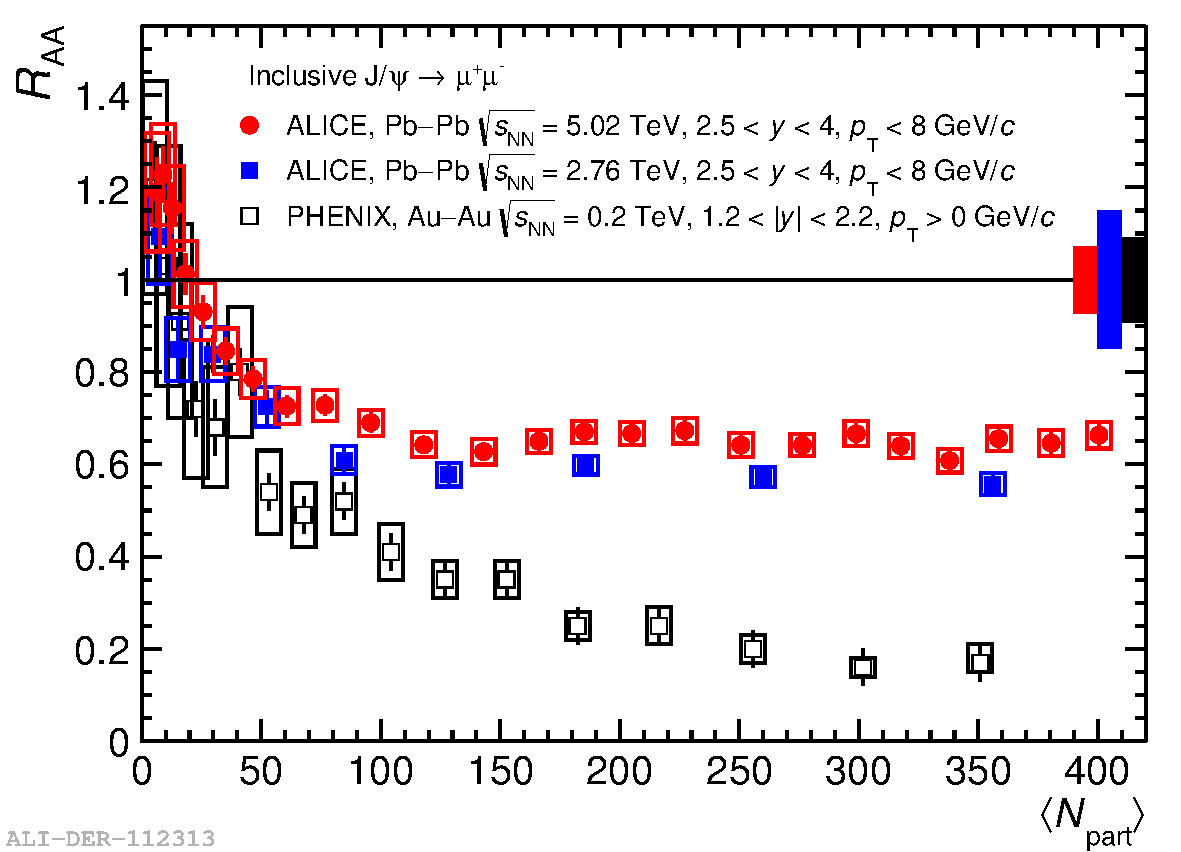
\includegraphics[width=0.8\linewidth]{Chapters/Analysis/Figs/2016-Sep-15-RAA_centr_Alice5_Alice276_Phenix.pdf}
\caption{$J/\psi$ nuclear modification factor measured by PHENIX (RHIC) at $\sqrt{s_{_{\rm NN}}}=200$ GeV (open black) and by ALICE at the LHC at $\sqrt{s_{_{\rm NN}}}=2.76$ and $5.02 \rm{TeV}$ (blue and red, respectively), as a function of the number of participant nucleons. The RHIC points appear systematically below ALICE ones over $<N_{part}>=50$, indicating a much lower suppression at LHC in the most central collisions. The two ALICE series appear to be in agreement over the whole centrality spectrum despite a factor ~$\times2$ for $\sqrt{s_{_{\rm NN}}}$. }
\label{fig:LHC_RHIC_jpsi}
\end{center}
\end{figure}

\begin{figure}[!t]
\begin{center}
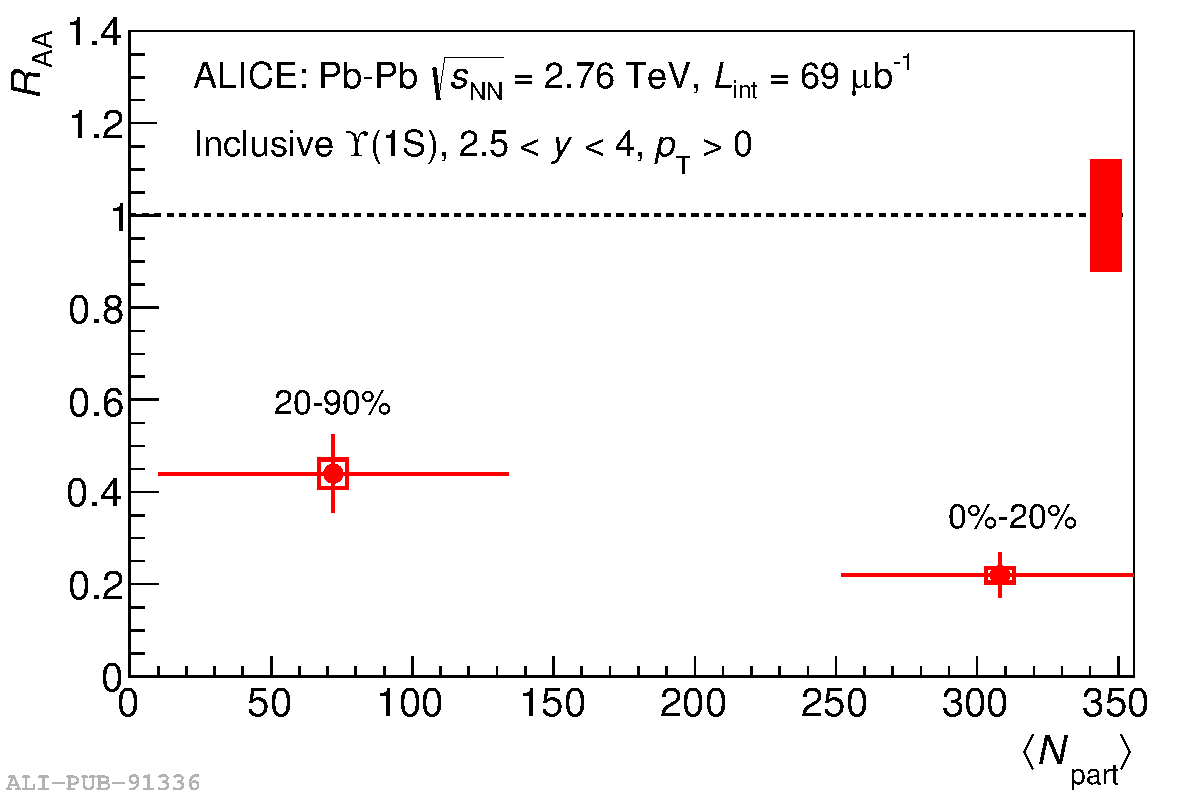
\includegraphics[width=0.8\linewidth]{Chapters/Analysis/Figs/2014-Dec-16-Raa_centr.pdf}
\caption{\upsi nuclear modification factor measured at the LHC by ALICE at $\sqrt{s_{_{\rm NN}}}=2.76$. Two centrality bins are shown, referring to the quoted centrality distribution percentiles.}
\label{fig:LHC_upsi}
\end{center}
\end{figure}

The theoretical models tuned to be able to describe the observed discrepancy included statistical regeneration mechanisms which were negligible at RHIC due to the much lower abundance of heavy quarks.
The provided models suggested that for \upsis production the regeneration effects would be still negligible, even at LHC collisions conditions, hence the bottomonium production studies were performed as well on the same data set.
As one can notice by performing a comparison between \ref{fig:LHC_RHIC_jpsi} and \ref{fig:LHC_upsi} the \upsi $R_{\rm{AA}}$ at $\sqrt{s_{_{\rm NN}}}=2.76$ appears to be similar to the $J/\psi$ one, measured at RHIC.
This observation is in agreement with the fact that the estimations of the total number of bottom quark pairs at the LHC and charm quark pairs at RHIC are almost aligned.
A strong suppression of the \upsis state in \pbpb collisions, with respect to properly scaled measurements from pp collisions, has been observed at $\sqrt{s_{_{\rm NN}}}=2.76$ \rm{TeV} by ALICE \cite{Abelev:2014nua} and CMS \cite{Chatrchyan:2012lxa,Khachatryan:2016xxp}, in the rapidity ranges $2.5<y<4$ and $|y|<2.4$, respectively \ref{fig:ALICE_CMS_upsi}. 

\begin{figure}[!t]
\begin{center}
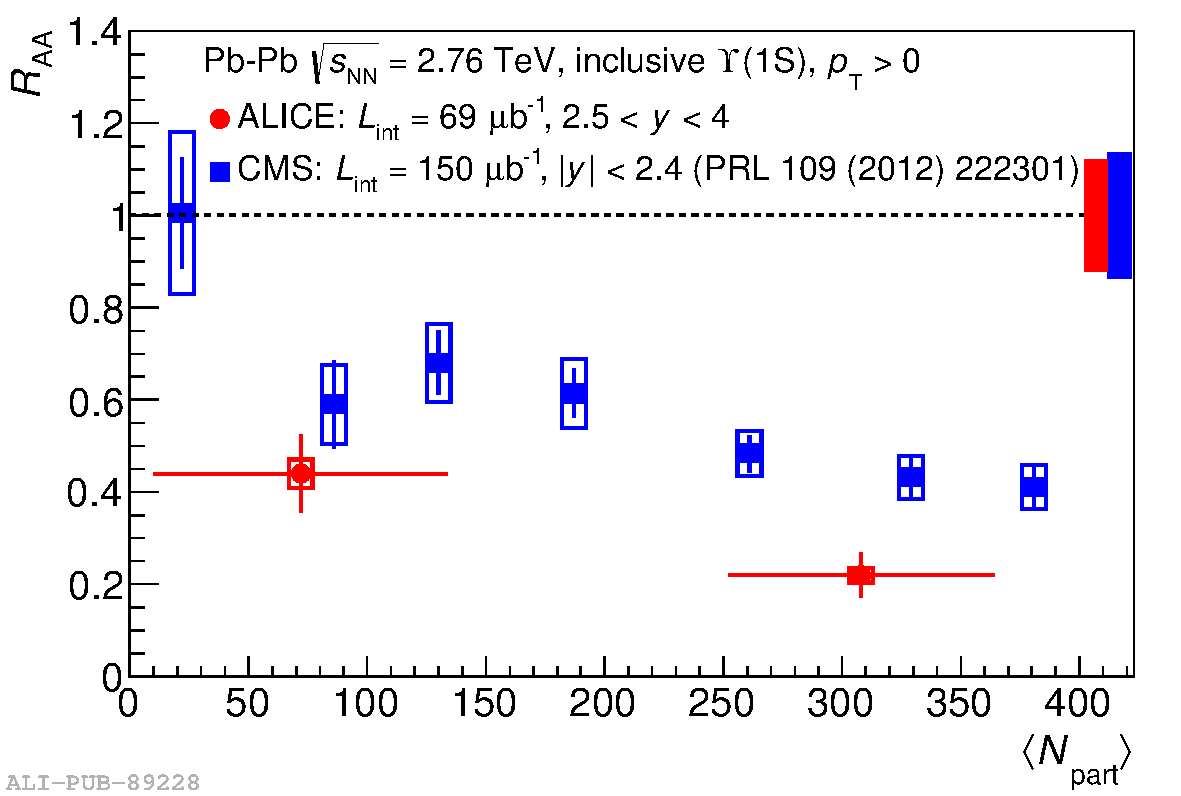
\includegraphics[width=0.47\linewidth]{Chapters/Analysis/Figs/2014-Nov-05-Raa_CMS_centr.pdf}
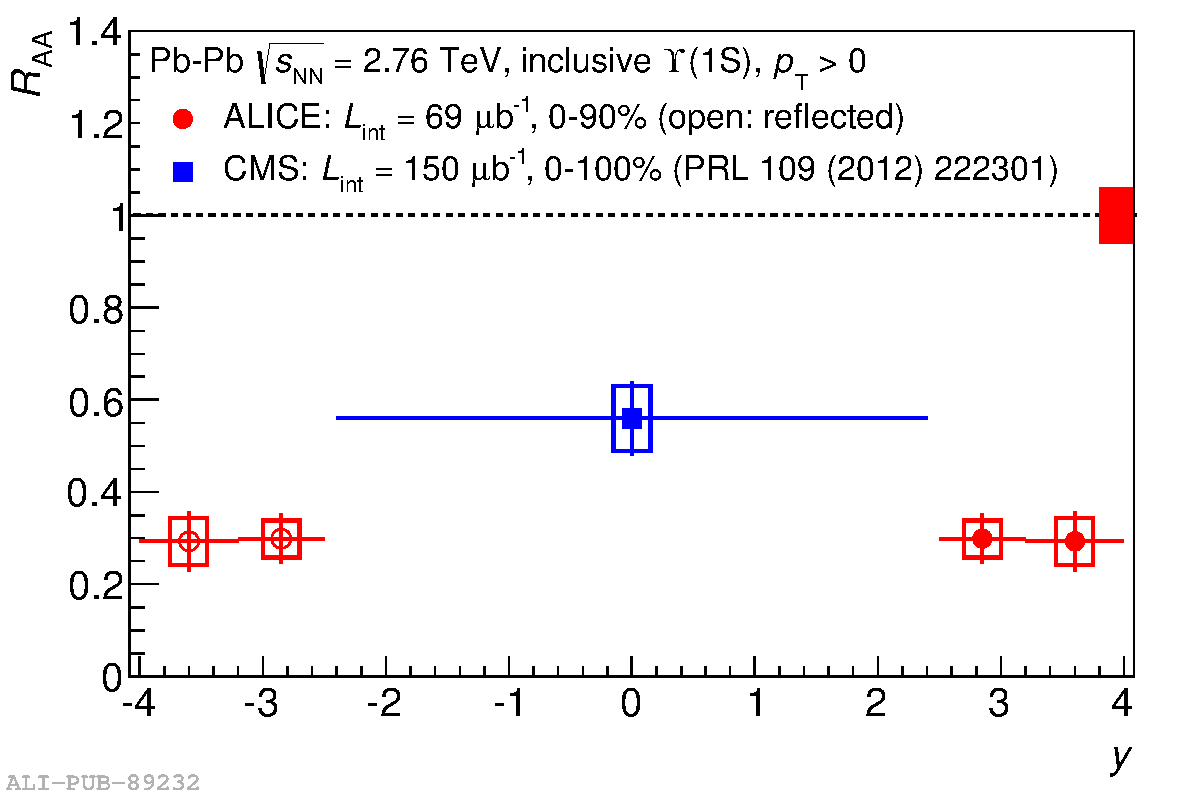
\includegraphics[width=0.47\linewidth]{Chapters/Analysis/Figs/2014-Nov-05-Raa_CMS_rap.pdf}
\caption{\upsis nuclear modification factor as a function of $<N_{part}>$ (left) and $y$ (right) measured by ALICE (red points, $2.5<y<4.0$) and CMS (blue points, $|y|<2.4$) at $\sqrt{s_{_{\rm NN}}}=2.76$ \rm{TeV}. A strong suppression is observed in both trends.}
\label{fig:ALICE_CMS_upsi}
\end{center}
\end{figure}

The suppression increases with the centrality of the collision, reaching about 60\% and 80\% for the most central collisions at mid-~\cite{Khachatryan:2016xxp} and forward rapidity~\cite{Abelev:2014nua}, respectively. 
Moreover, the \upsiss suppression reaches about 90\% and for \upsisss data are compatible with a complete suppression \cite{Khachatryan:2016xxp}. 
As a function of \pt the \upsis \raa, measured for $p_{\rm T}<20$ GeV/$c$ by CMS~\cite{Khachatryan:2016xxp}, is compatible with a constant value. 
When considering the $y$-dependence resulting from the comparison of ALICE and CMS results, there is an indication for a stronger suppression at forward $y$.
Transport models \cite{Zhou:2014kka,Du:2017qkv} fairly reproduce the experimental observations of CMS, while they tend to overestimate the $R_{\rm AA}$ values measured by ALICE. 
Similar conclusions can be obtained in the frame of an anisotropic hydrodynamic model \cite{Krouppa:2017jlg}. 
The comparison between $J/\psi$ and \upsis measurements performed by ALICE denotes a much stronger suppression for the former ($>3\sigma$) in the most central collisions \ref{fig:ALICE_jpsi_upsi}.

\begin{figure}[!t]
\begin{center}
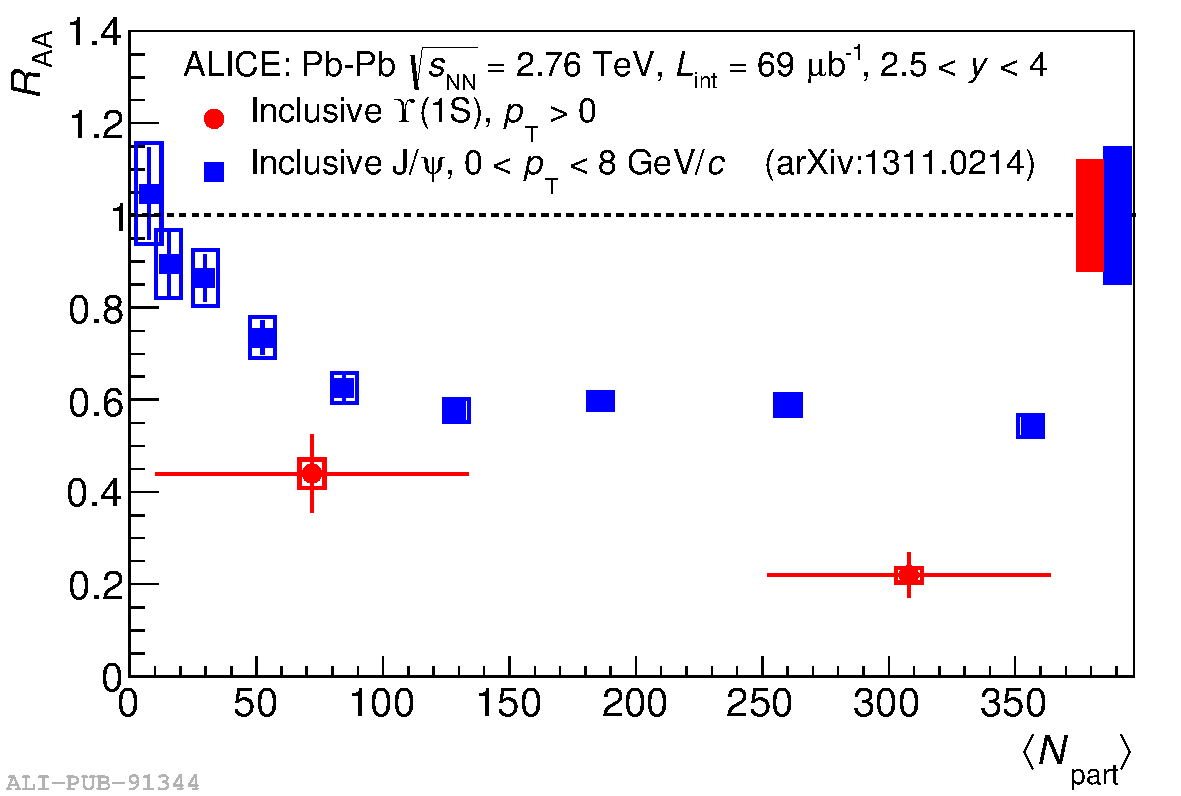
\includegraphics[width=0.8\linewidth]{Chapters/Analysis/Figs/2014-Dec-16-Raa_Jpsi_centr.pdf}
\caption{$J/\psi$ (blue) and \upsis (red) nuclear modification factor as a function of $<N_{part}>$ measured by ALICE at forward rapidity ($2.5<y<4.0$) at $\sqrt{s_{_{\rm NN}}}=2.76$ \rm{TeV}. The \upsis measurements are systematically and significantly below the $J/\psi$ points.}
\label{fig:ALICE_jpsi_upsi}
\end{center}
\end{figure}

The bottomonium suppression due to the QGP should be disentangled from the suppression due to Cold Nuclear Matter (CNM) effects, such as the nuclear modification of the parton distribution functions due to shadowing \cite{Eskola:1998df,Eskola:2009uj}, as well as parton energy loss \cite{Arleo:2012rs}.
These effects on the bottomonium production were studied in \ppb collisions by ALICE \cite{Abelev:2014oea} and LHCb \cite{Aaij:2014mza}, which reported for the \upsis a nuclear modification factor slightly lower than unity at forward rapidity and compatible with unity at backward rapidity, although with significant uncertainties \ref{fig:ALICE_pPb_jpsi_upsi}.
As a side note, in both rapidity ranges the compatibility between $J/\psi$ and \upsis is verified, suggesting a similar CNM effects contribution for charmonium and bottomonium.

\begin{figure}[!t]
\begin{center}
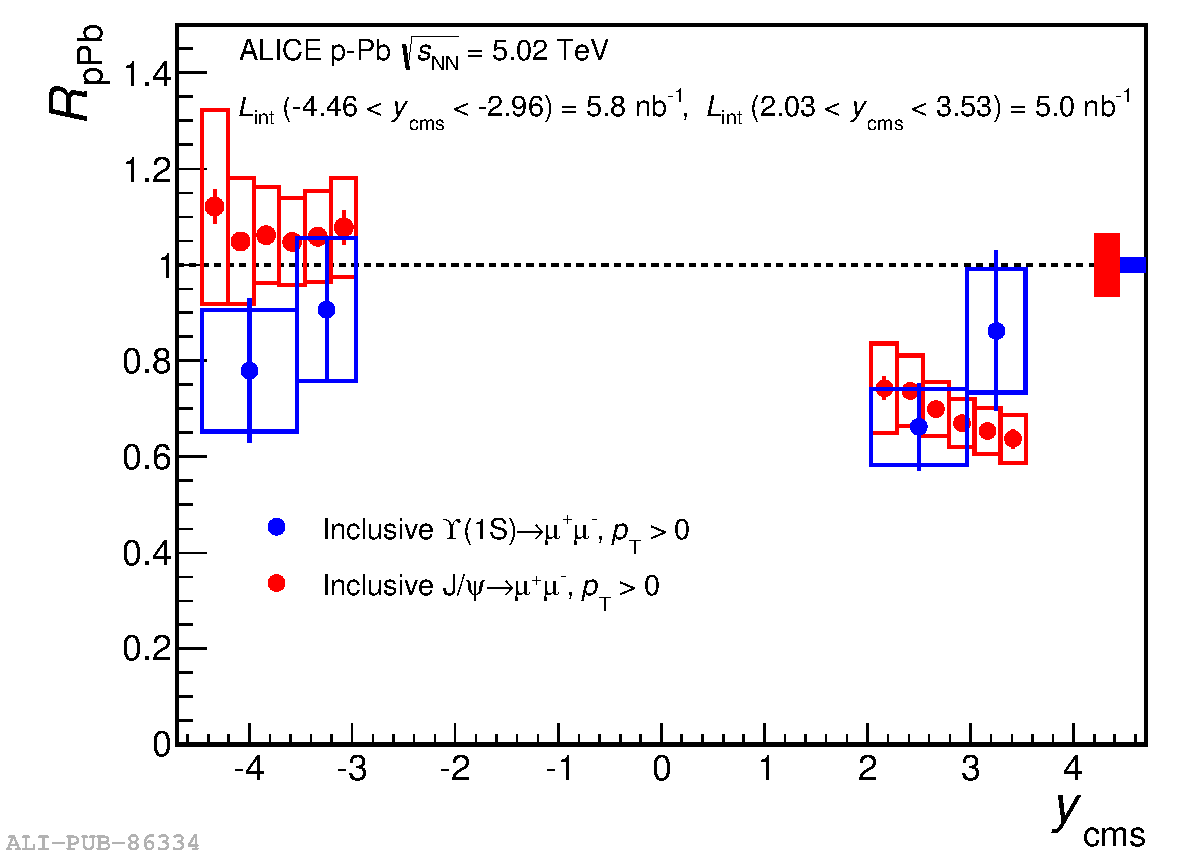
\includegraphics[width=0.8\linewidth]{Chapters/Analysis/Figs/2014-Oct-08-RpPb_Ups_Jpsi_b.pdf}
\caption{$J/\psi$ (red) and \upsis (blue) nuclear modification factor as a function of $y$ measured by ALICE is p-Pb collisions ($-4.46<y<-2.96$ and $2.03<y<3.53$) at $\sqrt{s_{_{\rm NN}}}=5.02$ \rm{TeV}. The \upsis measurements compatible with unity at backward rapidity and show partial suppression at forward rapidity. In both cases the \upsis measurements are compatible with $J/\psi$ ones.}
\label{fig:ALICE_pPb_jpsi_upsi}
\end{center}
\end{figure}

$p-Pb$ collisions are the CNM baseline since the achieved energy density is not enough to cause QGP production, but the nucleons of the colliding nuclei might be perturbed by the others.
Recently, ATLAS results indicate a significant suppression of the \upsis around mid-rapidity~\cite{Aaboud:2017cif}.  
Additional measurements at forward/backward rapidity with higher statistics, are needed to fully constrain the models and perform a meaningful extrapolation of CNM effects to \pbpb collisions.

\section{The Large Hadron Collider}
The Large Hadron Collider (LHC) is the most powerful particle accelerator ever built.
It is the largest element of the CERN acceleration facility and has been placed in the same $27km$ long tunnel previously used for the Large Electron Positron collider (LEP) placed between $45$ and $170m$ underground \ref{fig:accelerators}.
Some of the previous CERN accelerators are connected together and now used as pre acceleration steps for the final LHC injection.

\begin{figure}[!t]
\begin{center}
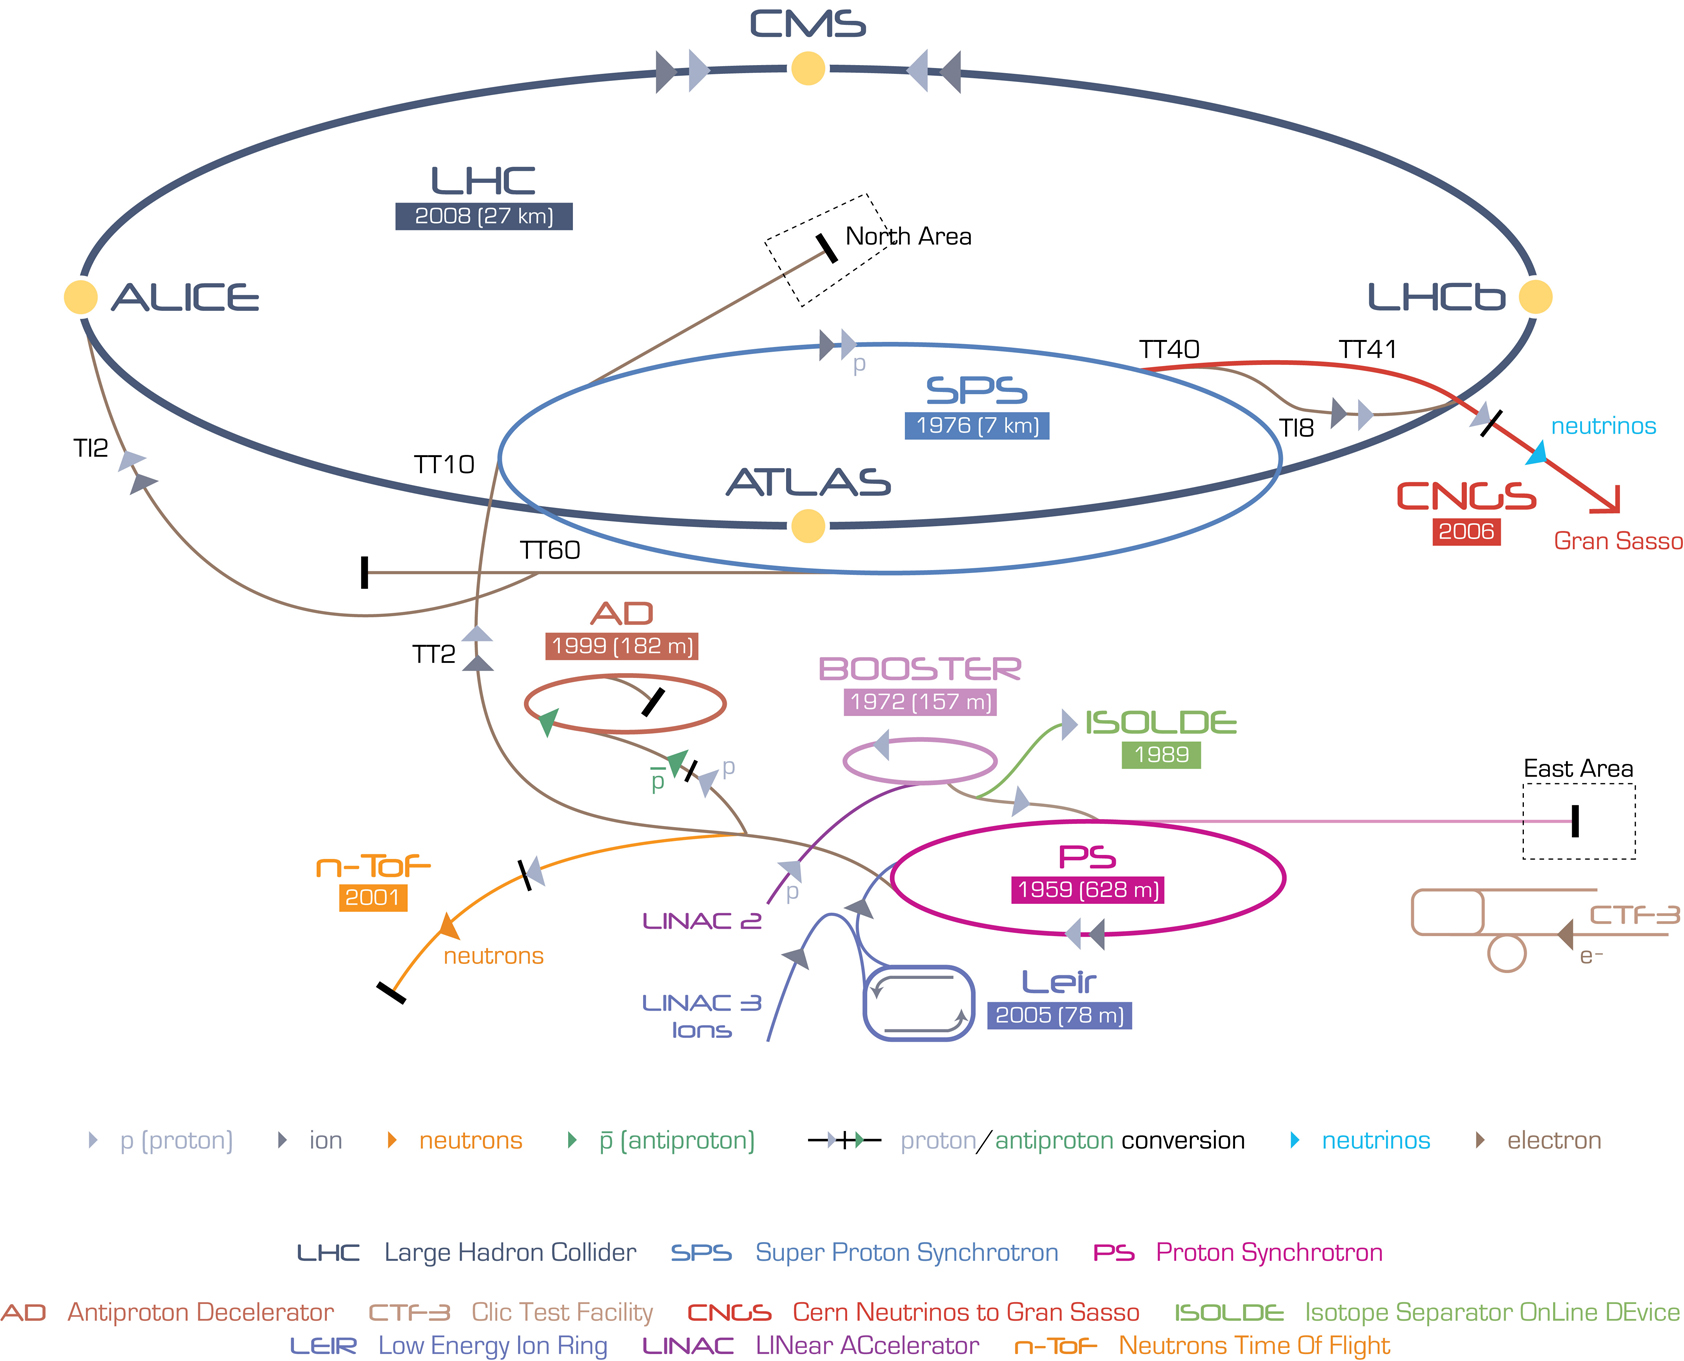
\includegraphics[width=\linewidth]{Chapters/Introduction/Figs/Cern-Accelerator-Complex.jpg}
\caption{Schematic representation of the CERN accelerator complex.}
\label{fig:accelerators}
\end{center}
\end{figure}

The LHC allows one to perform proton-proton, proton-Pb and Pb-Pb collisions (and lately also Xe-Xe).
For what concerns the pre-acceleration of protons the CERN LInear ACcelerators (LINAC), the Proton Synchrotron Booster (PSB), the Proton Synchrotron (PS) and the Super Proton Synchrotron are used upstream the LHC.
The heavy nuclei are instead firstly produced, ionized and accelerated in the Low Energy Ion Ring (LEIR) and then injected directly in the PS-SPS chain.
Thanks to the superconducting magnets (dipoles, quadrupoles and higher order ones) protons and nuclei can be accelerated up to $14TeV$ and $5.5TeV$ respectively.
Along the LHC ring four main experiments are placed: ALICE (A Large Ion Collider Experiment), CMS (Compact Muon Solenoid), ATLAS (A Toroidal LHC ApparatuS) and LHCb (Large Hadron Collider beauty).

%********************************** %Third Section  *************************************
\section{ALICE experimental setup} %Section - 1.3
The main purpose of the ALICE experiment is the study of the physics of strongly interacting matter in ultra-relativistic heavy-ion collisions. It is also designed for proton-proton and proton-nucleus collisions which represent an important part of its physics program. The experiment itself can be divided into three main sectors:
\begin{itemize}
    \item global detectors are used for triggering, event characterization and beam luminosity measurements;
    \item central barrel detectors are embedded into a solenoid with a magnetic field of B = 0.5 T and are used for tracking and identification of charged particles and photons;
    \item muon spectrometer covers the forward region with respect to the interaction point and its detectors are designed for muon tracking and trigger.
\end{itemize}

\begin{figure}[!t]
\begin{center}
\includegraphics[width=\linewidth]{Chapters/Introduction/Figs/ALICE-Setup.jpg}
\caption{Schematic of ALICE detectors setup, with a maximised view of the innermost detectors.}
\label{fig:ALICEsetup}
\end{center}
\end{figure}

The detector is completed by an array of scintillators to trigger on cosmic rays.
A more detailed discussion of the ALICE detectors is reported in the following sections.

\subsection{Central barrel}
The mid rapidity section of the ALICE experimental apparatus is named central barrel.
It includes many detectors, each of them with different purposes.
The structure surrounds the interaction point, covering the pseudorapidity range $|\eta| < 0.9$, and it is inside the $0.5 T$ magnetic field generated by a warm solenoidal magnet originally employed by the L3 collaboration.

\subsubsection{Inner Tracking System (ITS)}
The ITS is the closest detector to the beam pipe of the ALICE apparatus.
Its purposes are the identification of primary collision vertexes, the reconstruction of secondary vertexes from heavy particles decays and the tracking and identification of low momentum particles.
The spatial resolution of the ITS is lower than $100\mu~m$.
It is completely made of silicon detectors, implemented using three technologies.
Six layers compose the ITS:
\begin{itemize}
    \item Silicon Pixel Detector (SPD): two layers located at 3.9 and 7.6 cm from the interaction point, they are important for a high spatial resolution and for their very fast response;
    \item Silicon Drift Detector (SDD) : two layers located at 15 and 23.9 cm from the interaction point, they provide a bi-dimensional spatial information with a lower resolution than SPD;
    \item Silicon Strip Detector (SSD) : two layers located at 38 and 43 cm from the interaction point, they provide a complementary information on track positions.
\end{itemize}


\begin{figure}[!h]
\begin{center}
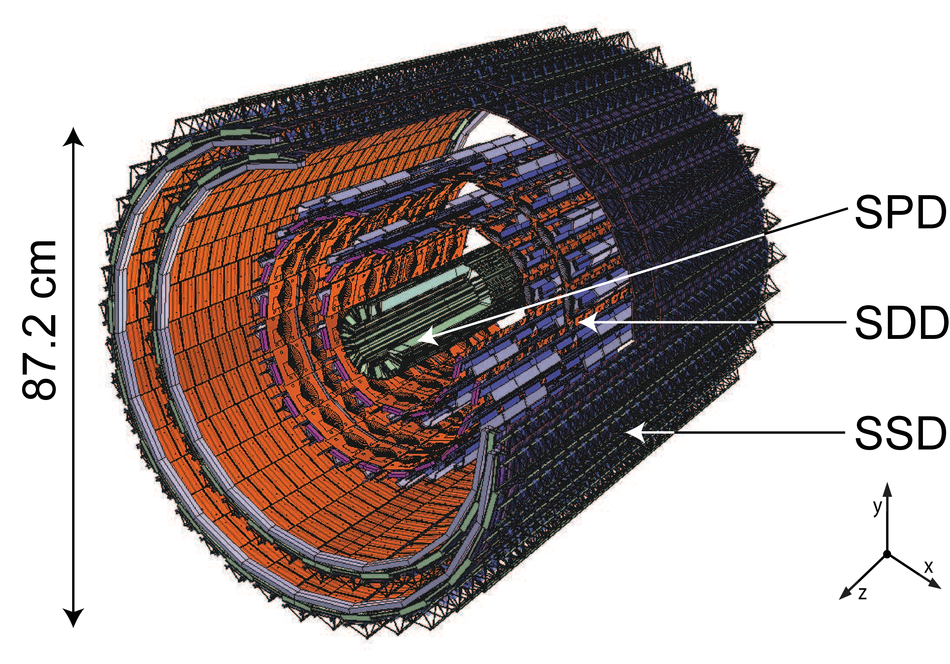
\includegraphics[width=0.7\linewidth]{Chapters/Introduction/Figs/its.png}
\caption{Schematic of the ALICE ITS.}
\label{fig:ITS}
\end{center}
\end{figure}

\subsubsection{Time Projection Chamber (TPC)}
The Time Projection Chamber is the main tracking detector of the central barrel.
It is a $88 m^3$ cylindrical detector filled with a gas mixture of $Ar$−$CO_2$ $(90-10\%)$.
Its volume is limited by two end-plates acting as segmented read-out electrodes. 
In addition an electrode is placed in the middle of the TPC, dividing it into two halves.
The ionizing particles crossing the detectors ionize the gaseous mixture.
The freed electrons drift towards the read-out electrodes.
As a result the side projection of the track is obtained directly from the electrodes, while the third coordinate of the points is obtained through the time of arrival of each segment.

\begin{figure}[!h]
\begin{center}
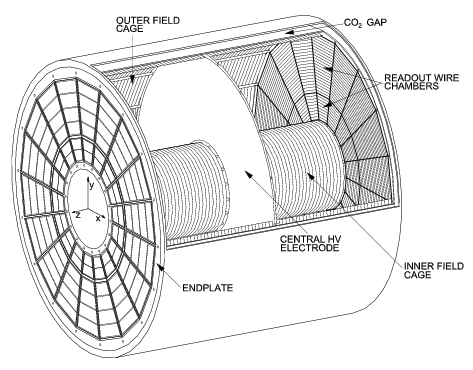
\includegraphics[width=0.7\linewidth]{Chapters/Introduction/Figs/tpc.png}
\caption{Representation of the TPC with some details of the layout.}
\label{fig:TPC}
\end{center}
\end{figure}

\subsubsection{Transition Radiation Detector (TRD)}
The Transition Radiation Detector is the main electron detector in ALICE.
It consists of six layers of multi-wire proportional chambers, filled with a mixture of $Xe$ and $CO_2$, equipped with a radiator made of optical fiber embedded in plastic foam directly glued on the electrode.
It is designed to provide charged-particle tracking, electron identification via transition radiation and pion rejection. 
The combination of ITS, TPC and TRD information provides a momentum resolution in the central barrel good enough to measure high pt tracks down to $100 GeV/c$ and a mass resolution about $100 MeV/c$.

\begin{figure}[!h]
\begin{center}
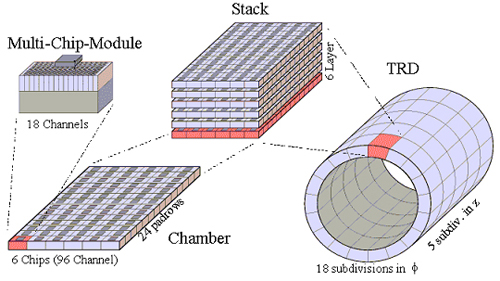
\includegraphics[width=0.7\linewidth]{Chapters/Introduction/Figs/trd.jpg}
\caption{Schematic of the ALICE TRD with an highlight on the modular struture of the detector.}
\label{fig:TRD}
\end{center}
\end{figure}

\subsubsection{Time Of Flight (TOF)}
The Time Of Flight detector is designed to identify charged particles with a momentum from $1 GeV/c$ to few $GeV/c$, extending the TPC particle identification capabilities. 
It is composed by multi-gap resistive plate chambers arranged into $18$ sectors in a cylindrical shell placed $3.7 m$ far from the beam pipe. 
The TOF provides the arrival time of a particle in the detector’s volume with a resolution of $80 ps$, completing the information gathered by TPC and TRD, in terms of identification of the detected particles, in particular separating $\pi/K$ up to $2.2 GeV/c$ and $K/p$ up to $4 GeV/c$.

\begin{figure}[!h]
\begin{center}
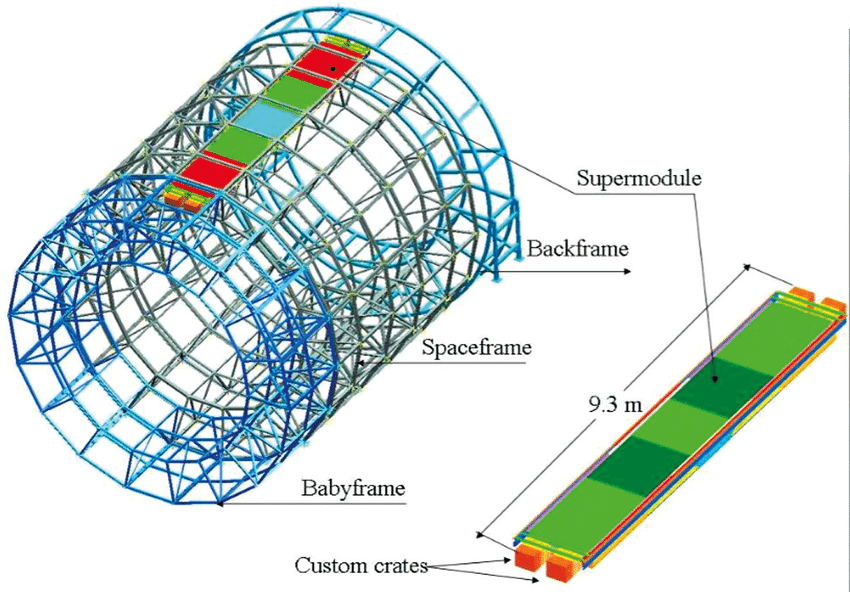
\includegraphics[width=0.7\linewidth]{Chapters/Introduction/Figs/tof.png}
\caption{Schematic of the ALICE TOF. A detector module is represented along with the support structure.}
\label{fig:TOF}
\end{center}
\end{figure}

\subsubsection{High Momentum Particle Identification Detector (HMPID)}
The main purpose of HMPID is to enhance the particle identification capability beyond the range allowed by ITS, TPC and TOF. 
It is based on proximity focusing Ring Imaging Cherenkov (RICH) counters and consists of seven modules mounted in an independent support cradle. 
When a fast charged particle traverses the $15 mm$ layer of liquid $C_6F_{14}$, Cherenkov photons are emitted and detected by the photon counter, which is a thin layer of $CsI$ deposited onto the pad cathode of multi-wire proportional chambers.

\begin{figure}[!h]
\begin{center}
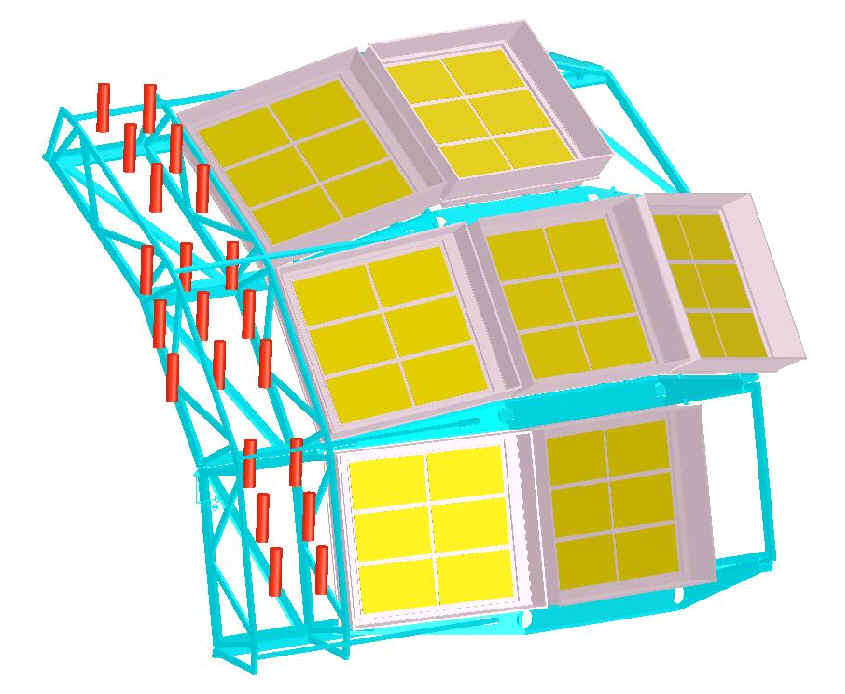
\includegraphics[width=0.4\linewidth]{Chapters/Introduction/Figs/hmpid.jpg}
\caption{The HMPID layout.}
\label{fig:HMPID}
\end{center}
\end{figure}

\subsubsection{PHOton Spectrometer (PHOS)}
The Photon Spectrometer is a high resolution electromagnetic spectrometer which consists of a highly segmented electromagnetic calorimeter of lead-tungstate crystals.
It is located on the bottom of the ALICE experimental apparatus, covering the pseudorapidity range $|\eta| < 0.12$, and it is designed for measuring photons and neutral mesons ($\pi_0$ and $\eta$) through their decays into two photons up to momenta about $10 GeV/c$.

\begin{figure}[!h]
\begin{center}
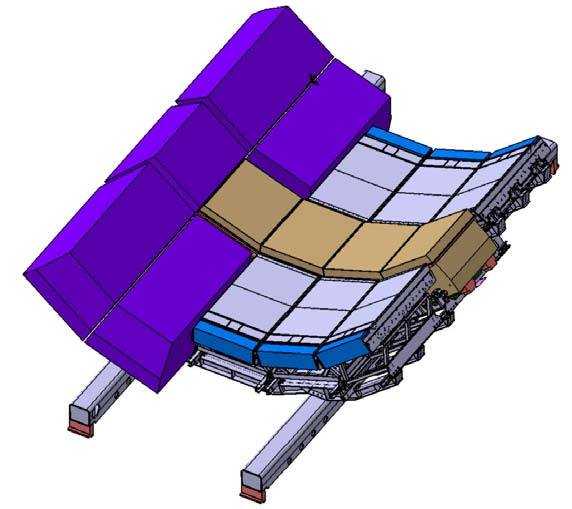
\includegraphics[width=0.5\linewidth]{Chapters/Introduction/Figs/phos.jpg}
\caption{The PHOS layout.}
\label{fig:PHOS}
\end{center}
\end{figure}

\subsubsection{ElectroMagnetic Calorimeter (EMCal)}
Positioned on the top of the ALICE structure, close to the solenoid coils, EMCal is designed to study jet quenching and it is used for triggering on photons, electrons and jets.
It is composed by 1152 towers of lead scintillators wiht photomultiplier readout and it covers a pseudo-rapidity range of $|\eta| < 0.7$.

\begin{figure}[!h]
\begin{center}
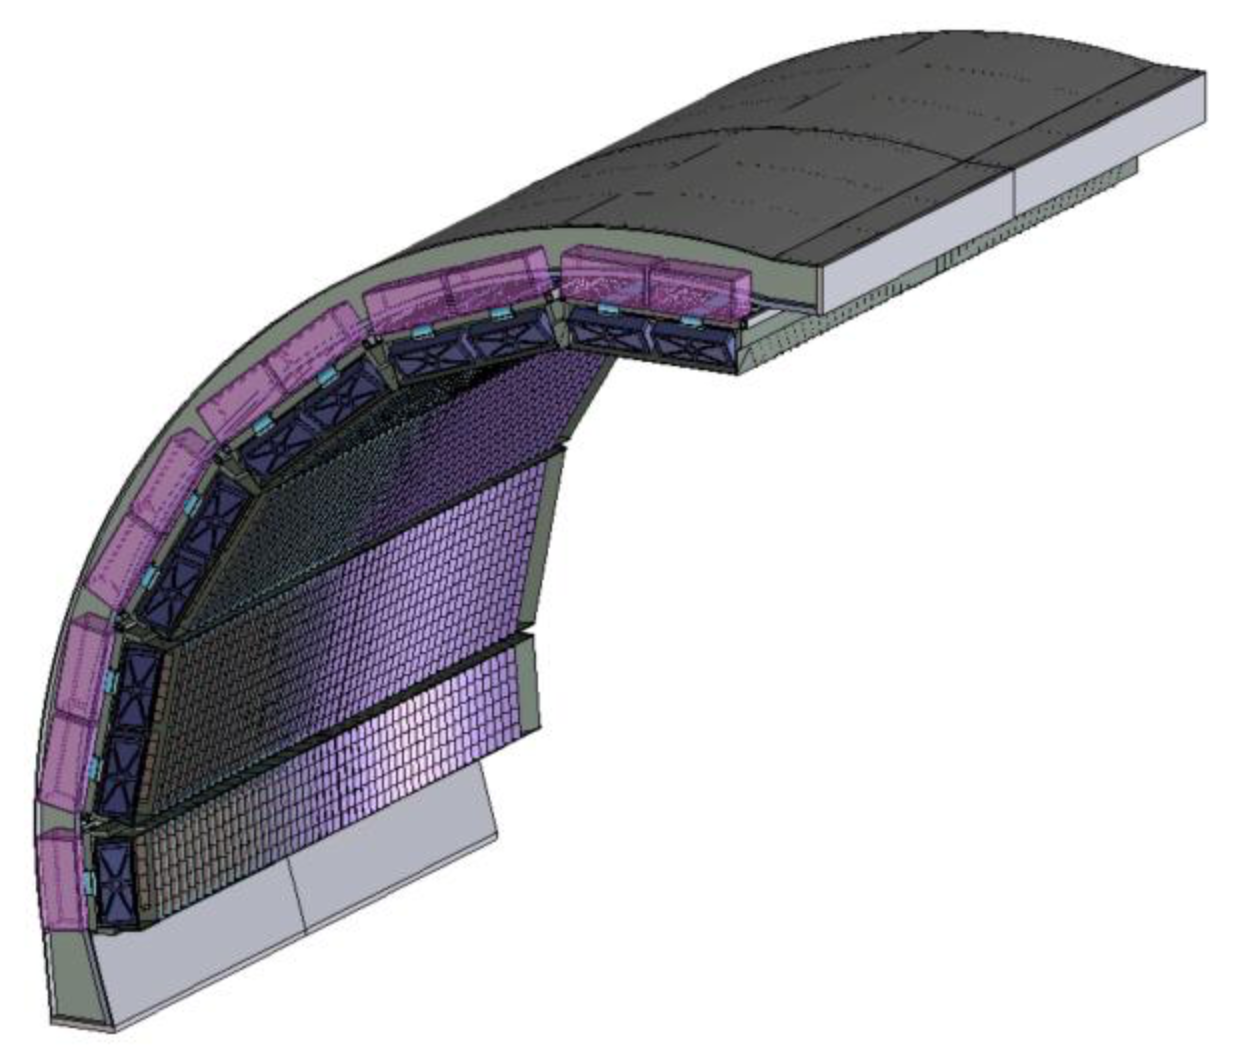
\includegraphics[width=0.5\linewidth]{Chapters/Introduction/Figs/emcal.png}
\caption{The EMCal layout.}
\label{fig:EMCAL}
\end{center}
\end{figure}

\subsection{Muon spectrometer}
The Muon Spectrometer is designed to measure muon production from the decays of quarkonia ($J/\psi$ , $\psi(2S)$ , $\Upsilon(1S)$, $\Upsilon(2S)$ and $\Upsilon(3S)$), low mass vector mesons ($\rho$, $\omega$ and $\phi$), heavy flavor hadrons and $W^\pm$ and $Z^0$ bosons. 
The detector is located in the pseudorapidity region $−4.0 < \eta < −2.5$ and it has a total length of $17 m$. 
It is composed by a system of passive absorbers, a dipole magnet, a muon tracker, an iron wall and a muon trigger system. 
The main components of the Muon Spectrometer will be discussed with more details in the following.

\begin{figure}[!h]
\begin{center}
\includegraphics[width=\linewidth]{Chapters/Introduction/Figs/spectro.png}
\caption{Schematic representation of ALICE with highlighted muon spectrometer components.}
\label{fig:spectro}
\end{center}
\end{figure}

\subsubsection{Absorbers system}
The Muon Spectrometer requires some shielding to reduce the otherwise large background produced expecially in nucleus-nucleus collisions.
For this reason it is equipped with a system of absorbers:
\begin{itemize}
    \item front absorber: this absorber is located inside the central barrel as close as $90 cm$ from the interaction point. The purpose of the front absorber is to filter out hadrons and to reduce the background generated by pions and kaons decays. The materials the front absorber is made of have been chosen to limit the multiple scattering of muons and leptons in general. The section of the front absorber placed closest to the interaction point is made of carbon to limit multiple scattering thanks to the low Z. The next sections of the absorber are composed of concrete to absorb secondary particles and low energy protons and neutrons. The whole absorber is coated of lead and boronated polyethilene to avoid decay products recoils in the TPC;
    \item beam shield: the beam pipe is layered with this shielding made of tungsten, lead and stainless steel to shield the muon spectrometer from the particles produced in the interactions between low angle particles and gas residuals inside the beam pipe;
    \item iron wall: this $1.2m$ thick absorber is placed between two detector systems and acts as a filter capable of absorbing everything but muons and other penetrating particles;
    \item rear absorber: an additional passive element has been installed around the connection hole between the experiment cave with the LHC tunnel in order to further remove products of gas interaction.
\end{itemize}

\subsubsection{Dipole magnet}
Located at $7m$ from the interaction point, the dipole magnet is used to determine the momentum and the electric charge of particles produced in the interaction point.
The value of the magnetic field provided (the magnetic flux density is $0.7T$ and the integrated value is $3T\cdot~m$) is defined by requirements of mass resolution.
The magnetic field is perpendicular to the beam pipe.
The definition of bending and non-bending planes follows the magnetic field direction.
The plane $zy$ is defined as the bending plane, since the dipole action deviates muons in this direction, and the plane $xz$ as the non-bending plane.

\begin{figure}[th]
\begin{center}
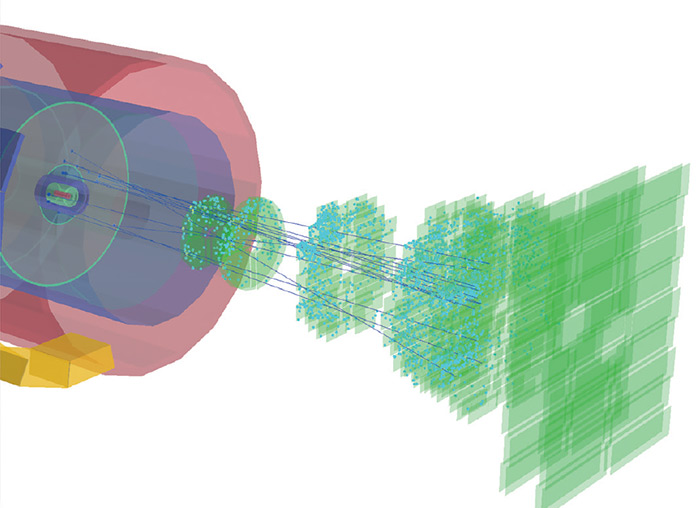
\includegraphics[width=\linewidth]{Chapters/Introduction/Figs/muon_mtr_mch.jpg}
\caption{Digital representation of the layout of the muon chambers and muon trigger system, shown in green.}
\label{fig:mch_mtr}
\end{center}
\end{figure}

\subsubsection{Muon Tracker or Muon Chambers (MCH)}
The tracking system is made of $10$ multi wire proportional chambers arranged in $5$ stations of $2$ chambers each.
The anode is implemented as wires placed between the readout sides, while the readout electrodes are strips or pads placed on the sides.
The produced electrons generate an avalanche drifting towards the nearest anode wire, and the resulting ion cloud induces a charge distribution on the cathode planes, allowing to determine the position of the track.
The size of the chambers depends on the spectrometer’s angular coverage, considering the deviation of muons by the magnetic field (because for this reason stations from 3 to 5 have larger dimensions).
The pad size of all the chambers is smaller close to the beam pipe, in order to take into account the higher density of particles produced in that region.
The spatial resolution is better than $2 mm$ and all the chambers are made of composite material ($< 3\%$ $X_0$ per chamber) to minimize the scattering of the muons in order to obtain the required resolution. 
To limit the occupation rate to a maximum of $5\%$ the full set of chambers has more than $1$ million channels.

\subsubsection{Muon Trigger (MTR)}
The muon trigger system is designed to tag high $p_T$ muons produced in heavy quarkonia and open heavy flavour mesons decays.
Thank to a configurable $p_T$ threshold, the system is able to provide trigger signals to select interesting events and to discard events with only low $p_T$ muons, which mainly come from pions and kaons decays.
The muon trigger system is composed of 72 Resistive Plate Chambers with $x-y$ read out, organized in $4$ planes paired in two stations to provide redundancy.
Each RPC consists of two planes, made of bakelite and separated by 2 mm of gas.
A charged particle passing through the gas ionizes it, causing the formation of an avalanche of secondary electrons, which are picked up by the copper strips placed outside the chambers.
The pattern of hit strips, gathered by the front-end electronics, is sent to the local trigger board which provides a first measure of muon momentum and gives the trigger decision.
The latter is performed considering the deviation of a track with respect to the track with infinite momentum ($p_T \rightarrow \infty$). The deviation has to be smaller than a certain value, which corresponds to the $p_T$ cut.